\documentclass[a4paper,10pt]{article}
\usepackage[margin=18mm,top=23mm,bottom=21mm]{geometry}
\usepackage{fontspec,amsmath,amssymb,mathtools,graphicx,xcolor,tikz,fancyhdr,needspace,array,longtable,booktabs,colortbl}
\setmainfont{DejaVu Sans}
\definecolor{navy}{HTML}{1E3A5F}
\definecolor{muted}{HTML}{475569}
\definecolor{pass}{HTML}{166534}
\definecolor{fail}{HTML}{B91C1C}
\pagestyle{fancy}\fancyhf{}\fancyhead[L]{\small\color{navy}mCalcCanvas | Composite Beam EC4}
\fancyhead[R]{\small CALC-EC4-01 | Rev C}
\fancyfoot[L]{\scriptsize Review preview from worksheet data — not an app PDF export}
\fancyfoot[R]{\small\thepage}
\setlength{\parindent}{0pt}\setlength{\parskip}{4pt}
\setlength{\headheight}{14pt}
\newsavebox{\eqbox}
\newcommand{\eq}[1]{\sbox{\eqbox}{$\displaystyle #1$}\ifdim\wd\eqbox>\linewidth\resizebox{\linewidth}{!}{\usebox{\eqbox}}\else\usebox{\eqbox}\fi}
\definecolor{light}{HTML}{F1F4F7}
\renewcommand{\headrulewidth}{0.5pt}
\newcommand{\sect}[1]{\Needspace{30mm}\vspace{10pt}\noindent\colorbox{navy}{\parbox{\dimexpr\linewidth-2\fboxsep}{\vspace{4pt}\color{white}\large\bfseries #1\vspace{4pt}}}\par\vspace{3pt}}
\begin{document}

{\small\color{muted}STRUCTURAL DESIGN WORKSHEET / CALC-EC4-01}\par
{\fontsize{25}{29}\selectfont\bfseries\color{navy}Composite beam}\par
{\Large\color{navy}EC4 calculation worksheet}\par
\vspace{5pt}
\begin{tabular*}{\linewidth}{@{\extracolsep{\fill}}lll@{}}
\textbf{8.0 m span} & \textbf{UB 406 $\times$ 178 $\times$ 60} & \textbf{150 mm solid slab}\\
Unpropped construction & S355 / C30/37 & Partial shear connection
\end{tabular*}\par
\vspace{8pt}\hrule\vspace{5pt}
{\small\textbf{Issue C / Presentation review.} Numerical content retained from the independently checked draft. Construction-stage stability and transverse reinforcement require revision.}\par
\sect{1. DESIGN BASIS}
{\small\color{muted}REVIEW DRAFT — engineering and layout approval; Singapore NA verification is outstanding.}\par
{\small\color{muted}SS EN 1994-1-1:2009; technical equations from EN 1994-1-1:2004. Solid slab; sagging UDL.}\par
{\small\color{muted}Simply supported, unpropped, symmetric rolled I-section; ductile studs; no applied axial force.}\par
{\small\color{muted}EC3 Class 1/2 plastic design. No openings, fatigue, fire, vibration or transverse slab design.}\par
{\small\color{muted}All displayed values are calculated by existing worksheet operators; no engine extension.}\par
{\small\color{muted}EN recommended factors below are explicit review inputs, not verified Singapore NA values.}\par
{\small\color{muted}The example retains failed checks. It is a reference calculation, not an approved beam design.}\par
\sect{2. INPUT PARAMETERS}
\Needspace{22mm}\vspace{8pt}{\normalsize\bfseries\color{navy}2.1 Geometry, materials and stages}\par
\Needspace{25mm}\begin{longtable}{@{}p{0.53\linewidth}p{0.43\linewidth}@{}}\rowcolor{light}\textbf{Parameter / reference} & \textbf{Definition / value}\\\midrule
{\small Span} & {\small $L\coloneq 8\,\mathrm{m}$}\\[5pt]
{\small Slab thickness} & {\small $h_c\coloneq 150\,\mathrm{mm}$}\\[5pt]
{\small Left / right beam spacing (symmetric example)} & {\small $s_b\coloneq 3\,\mathrm{m}$}\\[5pt]
{\small Outermost stud-row separation: single row} & {\small $b_0\coloneq 0\,\mathrm{mm}$}\\[5pt]
{\small Steel yield strength, tf < 16 mm} & {\small $f_y\coloneq 355\,\mathrm{MPa}$}\\[5pt]
{\small Steel elastic modulus} & {\small $E_a\coloneq 210\,\mathrm{GPa}$}\\[5pt]
{\small Steel shear modulus} & {\small $G_a\coloneq 81\,\mathrm{GPa}$}\\[5pt]
{\small Concrete C30/37, EC2 Table 3.1} & {\small $f_{ck}\coloneq 30\,\mathrm{MPa}$}\\[5pt]
{\small Concrete secant modulus, EC2 Table 3.1} & {\small $E_{cm}\coloneq 33\,\mathrm{GPa}$}\\[5pt]
{\small Reinforcement B500} & {\small $f_{sk}\coloneq 500\,\mathrm{MPa}$}\\[5pt]
{\small EN recommended factor — NA review required} & {\small $\gamma_C\coloneq 1.5$}\\[5pt]
{\small EN recommended factor — NA review required} & {\small $\gamma_S\coloneq 1.15$}\\[5pt]
{\small EN recommended factor — NA review required} & {\small $\gamma_V\coloneq 1.25$}\\[5pt]
{\small EN recommended factor — NA review required} & {\small $\gamma_{M0}\coloneq 1$}\\[5pt]
{\small EN recommended factor — NA review required} & {\small $\gamma_{M1}\coloneq 1$}\\[5pt]
{\small EN recommended factor — NA review required} & {\small $\gamma_G\coloneq 1.35$}\\[5pt]
{\small EN recommended factor — NA review required} & {\small $\gamma_Q\coloneq 1.5$}\\[5pt]\bottomrule\end{longtable}\Needspace{24mm}\begin{minipage}{\linewidth}{\small\bfseries\color{muted}EC4 §2.4.1.2(2): no additional EC2 alpha-cc factor}\par\vspace{3pt}{\small\eq{f_{cd}\coloneq  \frac{f_{ck}}{\gamma_C}}\par\vspace{2pt}\eq{=\frac{30\,\mathrm{MPa}}{1.5}}\par\vspace{2pt}\eq{\color{navy}=20\,\mathrm{MPa}}}\par\vspace{7pt}\end{minipage}\par
\Needspace{24mm}\begin{minipage}{\linewidth}{\small\bfseries\color{muted}Steel design yield strength}\par\vspace{3pt}{\small\eq{f_{yd}\coloneq  \frac{f_y}{\gamma_{M0}}}\par\vspace{2pt}\eq{=\frac{355\,\mathrm{MPa}}{1}}\par\vspace{2pt}\eq{\color{navy}=355\,\mathrm{MPa}}}\par\vspace{7pt}\end{minipage}\par
\Needspace{24mm}\begin{minipage}{\linewidth}{\small\bfseries\color{muted}Reinforcement design yield strength}\par\vspace{3pt}{\small\eq{f_{sd}\coloneq  \frac{f_{sk}}{\gamma_S}}\par\vspace{2pt}\eq{=\frac{500\,\mathrm{MPa}}{1.15}}\par\vspace{2pt}\eq{\color{navy}=434.783\,\mathrm{MPa}}}\par\vspace{7pt}\end{minipage}\par

\Needspace{22mm}\vspace{8pt}{\normalsize\bfseries\color{navy}2.2 Loads, programme and serviceability}\par
\Needspace{25mm}\begin{longtable}{@{}p{0.53\linewidth}p{0.43\linewidth}@{}}\rowcolor{light}\textbf{Parameter / reference} & \textbf{Definition / value}\\\midrule
{\small Wet RC density: includes reinforcement allowance} & {\small $\rho_c\coloneq 25\,\mathrm{kN/m^3}$}\\[5pt]
{\small Construction UDL, explicit project assumption} & {\small $q_{con}\coloneq 0.75\,\mathrm{kPa}$}\\[5pt]
{\small Removable formwork load, explicit assumption} & {\small $g_{form}\coloneq 0.5\,\mathrm{kPa}$}\\[5pt]
{\small Post-curing finishes / SDL} & {\small $g_{SDL}\coloneq 1.5\,\mathrm{kPa}$}\\[5pt]
{\small Final imposed load} & {\small $q_k\coloneq 3\,\mathrm{kPa}$}\\[5pt]
{\small Quasi-permanent factor, occupancy assumption} & {\small $\psi_2\coloneq 0.3$}\\[5pt]
{\small Creep coefficient, project assessment input} & {\small $\varphi\coloneq 2$}\\[5pt]
{\small Free shrinkage magnitude after composite activation} & {\small $\varepsilon_{cs}\coloneq 0.0003$}\\[5pt]
{\small Construction and final total deflection denominator} & {\small $r_{lim}\coloneq 250$}\\[5pt]\bottomrule\end{longtable}
{\small\color{muted}Construction load excludes local heaping, impact and pump loads; assess these separately.}\par
{\small\color{muted}EN 1990 §6.4.3 / Annex A1 and EN 1991-1-6: combinations need project/NA approval.}\par
{\small\color{muted}Formwork and construction imposed loads are removed before the final service condition.}\par
\sect{3. STEEL SECTION PROPERTIES}
{\small\color{muted}UB 406 x 178 x 60; published SCI section data, not a geometry-derived sharp-corner section.}\par
{\small\color{muted}Phase 1: native explicit inputs. UB table / lookup binding remains a future integration task.}\par
\Needspace{25mm}\begin{longtable}{@{}p{0.53\linewidth}p{0.43\linewidth}@{}}\rowcolor{light}\textbf{Parameter / reference} & \textbf{Definition / value}\\\midrule
{\small Published section property} & {\small $h_a\coloneq 406.4\,\mathrm{mm}$}\\[5pt]
{\small Published section property} & {\small $b_a\coloneq 177.9\,\mathrm{mm}$}\\[5pt]
{\small Published section property} & {\small $t_f\coloneq 12.8\,\mathrm{mm}$}\\[5pt]
{\small Published section property} & {\small $t_w\coloneq 7.9\,\mathrm{mm}$}\\[5pt]
{\small Published section property} & {\small $r\coloneq 10.2\,\mathrm{mm}$}\\[5pt]
{\small Published section property} & {\small $A_a\coloneq 7650\,\mathrm{mm^2}$}\\[5pt]
{\small Published section property} & {\small $I_a\coloneq 216000000\,\mathrm{mm^4}$}\\[5pt]
{\small Published section property} & {\small $I_z\coloneq 12000000\,\mathrm{mm^4}$}\\[5pt]
{\small Published section property} & {\small $W_{pl}\coloneq 1200000\,\mathrm{mm^3}$}\\[5pt]
{\small Published section property} & {\small $W_{el}\coloneq 1060000\,\mathrm{mm^3}$}\\[5pt]
{\small Published section property} & {\small $I_t\coloneq 333000\,\mathrm{mm^4}$}\\[5pt]
{\small Published section property} & {\small $I_w\coloneq 466000000000\,\mathrm{mm^6}$}\\[5pt]
{\small Published section property} & {\small $m_a\coloneq 60.1\,\mathrm{kg/m}$}\\[5pt]\bottomrule\end{longtable}\Needspace{24mm}\begin{minipage}{\linewidth}{\small\bfseries\color{muted}Steel self weight from section mass}\par\vspace{3pt}{\small\eq{g_a\coloneq  m_a\cdot9.81\,\mathrm{m/s^2}}\par\vspace{2pt}\eq{=(60.1\,\mathrm{kg}/\mathrm{m})\cdot 9.81(\mathrm{m}/\mathrm{s}^{2})}\par\vspace{2pt}\eq{\color{navy}=0.5896\,\mathrm{kN}/\mathrm{m}}}\par\vspace{7pt}\end{minipage}\par
\Needspace{24mm}\begin{minipage}{\linewidth}{\small\bfseries\color{muted}EC3 §6.2.6(3), conservative eta = 1.0}\par\vspace{3pt}{\small\eq{A_v\coloneq  A_a-2b_a t_f+(t_w+2r)t_f}\par\vspace{2pt}\eq{=7650\,\mathrm{mm}^{2}-2\cdot (0.1779\,\mathrm{m})\cdot (0.0128\,\mathrm{m})+(0.0079\,\mathrm{m}+2\cdot (0.0102\,\mathrm{m}))\cdot (0.0128\,\mathrm{m})}\par\vspace{2pt}\eq{\color{navy}=3458\,\mathrm{mm}^{2}}}\par\vspace{7pt}\end{minipage}\par

\Needspace{65mm}\begin{minipage}{\linewidth}\vspace{4pt}{\bfseries\color{navy}D02 — Composite section — geometry}\par

\centering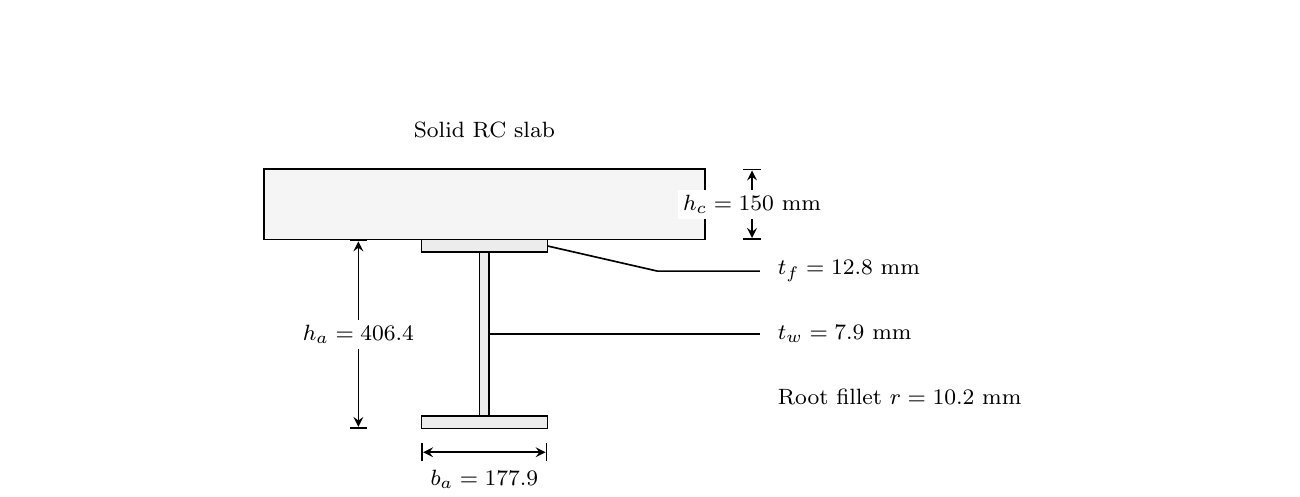
\begin{tikzpicture}[x=1cm,y=1cm,line width=.6pt,>=stealth,font=\fontsize{8.5}{10}\selectfont]\path[use as bounding box] (0,0) rectangle (15.8,5.6);\draw[fill=gray!15] (5,1) rectangle ++(1.6,.16);\draw[fill=gray!15] (5.74,1.16) rectangle ++(.12,2.08);\draw[fill=gray!15] (5,3.24) rectangle ++(1.6,.16);\draw[fill=gray!8] (3,3.4) rectangle (8.6,4.3);\draw[|<->|] (9.2,3.4)--(9.2,4.3) node[midway,fill=white,inner sep=2pt]{$h_c=150$ mm};\node at (5.8,4.8){Solid RC slab};\draw[|<->|] (4.2,1)--(4.2,3.4) node[midway,fill=white,inner sep=2pt]{$h_a=406.4$};\draw[|<->|] (5,0.7)--(6.6,0.7) node[midway,below=3pt]{$b_a=177.9$};\draw (6.6,3.32)--(8,3)--(9.3,3);\node[anchor=west] at (9.4,3){$t_f=12.8$ mm};\draw (5.86,2.2)--(8,2.2)--(9.3,2.2);\node[anchor=west] at (9.4,2.2){$t_w=7.9$ mm};\node[anchor=west] at (9.4,1.4){Root fillet $r=10.2$ mm};\node at (7.9,-.15){Dimensions in mm; section schematic; fillets omitted.};\end{tikzpicture}\end{minipage}\par\vspace{5pt}

\sect{4. STRUCTURAL ANALYSIS}
\Needspace{24mm}\begin{minipage}{\linewidth}{\small\bfseries\color{muted}Wet slab line load}\par\vspace{3pt}{\small\eq{g_c\coloneq  \rho_c h_c s_b}\par\vspace{2pt}\eq{=(25\,\mathrm{kN}/\mathrm{m}^{3})\cdot (0.15\,\mathrm{m})\cdot (3\,\mathrm{m})}\par\vspace{2pt}\eq{\color{navy}=11.25\,\mathrm{kN}/\mathrm{m}}}\par\vspace{7pt}\end{minipage}\par
\Needspace{24mm}\begin{minipage}{\linewidth}{\small\bfseries\color{muted}Permanent final line load}\par\vspace{3pt}{\small\eq{g_k\coloneq  g_a+g_c+g_{SDL}s_b}\par\vspace{2pt}\eq{=0.5896\,\mathrm{kN}/\mathrm{m}+11.25\,\mathrm{kN}/\mathrm{m}+(1.5\,\mathrm{kPa})\cdot (3\,\mathrm{m})}\par\vspace{2pt}\eq{\color{navy}=16.34\,\mathrm{kN}/\mathrm{m}}}\par\vspace{7pt}\end{minipage}\par
\Needspace{24mm}\begin{minipage}{\linewidth}{\small\bfseries\color{muted}Construction ULS, transient assumed combination}\par\vspace{3pt}{\small\eq{w_{1.Ed}\coloneq  \gamma_G(g_a+g_c+g_{form}s_b)+\gamma_Q q_{con}s_b}\par\vspace{2pt}\eq{=1.35(0.5896\,\mathrm{kN}/\mathrm{m}+11.25\,\mathrm{kN}/\mathrm{m}+(0.5\,\mathrm{kPa})\cdot (3\,\mathrm{m}))+1.5\cdot (0.75\,\mathrm{kPa})\cdot (3\,\mathrm{m})}\par\vspace{2pt}\eq{\color{navy}=21.383\,\mathrm{kN}/\mathrm{m}}}\par\vspace{7pt}\end{minipage}\par
\Needspace{24mm}\begin{minipage}{\linewidth}{\small\bfseries\color{muted}Final ULS, one leading variable action}\par\vspace{3pt}{\small\eq{w_{Ed}\coloneq  \gamma_G g_k+\gamma_Q q_k s_b}\par\vspace{2pt}\eq{=1.35\cdot (16.34\,\mathrm{kN}/\mathrm{m})+1.5\cdot (3\,\mathrm{kPa})\cdot (3\,\mathrm{m})}\par\vspace{2pt}\eq{\color{navy}=35.558\,\mathrm{kN}/\mathrm{m}}}\par\vspace{7pt}\end{minipage}\par
\Needspace{24mm}\begin{minipage}{\linewidth}{\small\bfseries\color{muted}Reaction / maximum shear, UDL}\par\vspace{3pt}{\small\eq{V_{1.Ed}\coloneq  \frac{w_{1.Ed}L}{2}}\par\vspace{2pt}\eq{=\frac{(21.383\,\mathrm{kN}/\mathrm{m})\cdot (8\,\mathrm{m})}{2}}\par\vspace{2pt}\eq{\color{navy}=85.534\,\mathrm{kN}}}\par\vspace{7pt}\end{minipage}\par
\Needspace{24mm}\begin{minipage}{\linewidth}{\small\bfseries\color{muted}Midspan maximum sagging moment, UDL}\par\vspace{3pt}{\small\eq{M_{1.Ed}\coloneq  \frac{w_{1.Ed}L^2}{8}}\par\vspace{2pt}\eq{=\frac{(21.383\,\mathrm{kN}/\mathrm{m})\cdot (8\,\mathrm{m})^{2}}{8}}\par\vspace{2pt}\eq{\color{navy}=171.067\,\mathrm{kN}\cdot \mathrm{m}}}\par\vspace{7pt}\end{minipage}\par
\Needspace{24mm}\begin{minipage}{\linewidth}{\small\bfseries\color{muted}Reaction / maximum shear, UDL}\par\vspace{3pt}{\small\eq{V_{2.Ed}\coloneq  \frac{w_{Ed}L}{2}}\par\vspace{2pt}\eq{=\frac{(35.558\,\mathrm{kN}/\mathrm{m})\cdot (8\,\mathrm{m})}{2}}\par\vspace{2pt}\eq{\color{navy}=142.234\,\mathrm{kN}}}\par\vspace{7pt}\end{minipage}\par
\Needspace{24mm}\begin{minipage}{\linewidth}{\small\bfseries\color{muted}Midspan maximum sagging moment, UDL}\par\vspace{3pt}{\small\eq{M_{2.Ed}\coloneq  \frac{w_{Ed}L^2}{8}}\par\vspace{2pt}\eq{=\frac{(35.558\,\mathrm{kN}/\mathrm{m})\cdot (8\,\mathrm{m})^{2}}{8}}\par\vspace{2pt}\eq{\color{navy}=284.467\,\mathrm{kN}\cdot \mathrm{m}}}\par\vspace{7pt}\end{minipage}\par

{\small\color{muted}Envelope: M(x) = w x (L-x)/2; V(x) = w (L/2-x), separately for each load stage.}\par
\Needspace{65mm}\begin{minipage}{\linewidth}\vspace{4pt}{\bfseries\color{navy}D01 — UDL, reactions and span}\par

\centering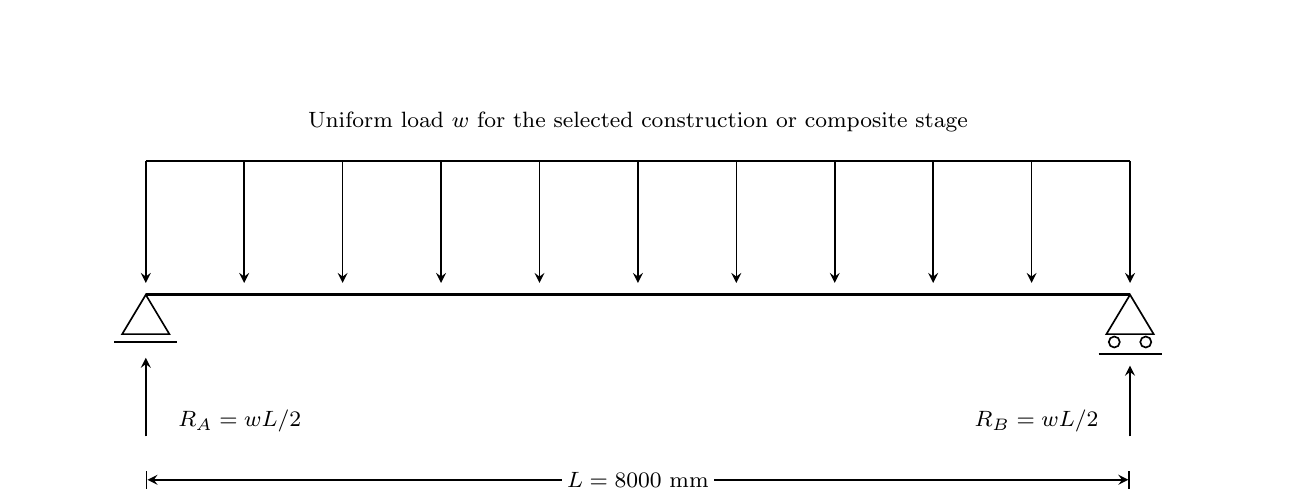
\begin{tikzpicture}[x=1cm,y=1cm,line width=.6pt,>=stealth,font=\fontsize{8.5}{10}\selectfont]\path[use as bounding box] (0,0) rectangle (15.8,5.6);\draw[line width=1pt] (1.5,2.7)--(14,2.7);
\draw (1.5,2.7)--(1.2,2.2)--(1.8,2.2)--cycle;\draw (14,2.7)--(13.7,2.2)--(14.3,2.2)--cycle;
\draw (13.8,2.1) circle (.07);\draw (14.2,2.1) circle (.07);
\draw (1.1,2.1)--(1.9,2.1);\draw (13.6,1.95)--(14.4,1.95);
\draw (1.5,4.4)--(14,4.4);\foreach \x in {1.5,2.75,...,14}{\draw[->] (\x,4.4)--(\x,2.85);}
\node at (7.75,4.9){Uniform load $w$ for the selected construction or composite stage};
\draw[->] (1.5,.9)--(1.5,1.9);\draw[->] (14,.9)--(14,1.8);
\node[anchor=east] at (3.6,1.1){$R_A=wL/2$};\node[anchor=west] at (11.9,1.1){$R_B=wL/2$};\draw[|<->|] (1.5,0.35)--(14,0.35) node[midway,fill=white,inner sep=2pt]{$L=8000$ mm};\end{tikzpicture}\end{minipage}\par\vspace{5pt}

\sect{5. CONSTRUCTION STAGE — STEEL ONLY}
{\small\color{muted}EC3 §5.5 / Table 5.2: bare steel section in major-axis bending, no axial force.}\par
\Needspace{24mm}\begin{minipage}{\linewidth}{\small\bfseries\color{muted}Material parameter}\par\vspace{3pt}{\small\eq{\varepsilon\coloneq  \sqrt{\frac{235\,\mathrm{MPa}}{f_y}}}\par\vspace{2pt}\eq{=\sqrt{\frac{235\mathrm{MPa}}{355\,\mathrm{MPa}}}}\par\vspace{2pt}\eq{\color{navy}=0.8136}}\par\vspace{7pt}\end{minipage}\par
\Needspace{24mm}\begin{minipage}{\linewidth}{\small\bfseries\color{muted}Flange outstand slenderness}\par\vspace{3pt}{\small\eq{\beta_f\coloneq  \frac{b_a-t_w-2r}{2t_f\varepsilon}}\par\vspace{2pt}\eq{=\frac{0.1779\,\mathrm{m}-0.0079\,\mathrm{m}-2\cdot (0.0102\,\mathrm{m})}{2\cdot (0.0128\,\mathrm{m})\cdot 0.8136}}\par\vspace{2pt}\eq{\color{navy}=7.182}}\par\vspace{7pt}\end{minipage}\par
\Needspace{25mm}\begin{longtable}{@{}p{0.53\linewidth}p{0.43\linewidth}@{}}\rowcolor{light}{\small Class 1 flange limit} & {\small $\beta_{f}=7.182\;\le\;9\quad\text{\color{pass}PASS}$}\\[5pt]\end{longtable}\Needspace{24mm}\begin{minipage}{\linewidth}{\small\bfseries\color{muted}Web slenderness in pure bending}\par\vspace{3pt}{\small\eq{\beta_w\coloneq  \frac{h_a-2t_f-2r}{t_w\varepsilon}}\par\vspace{2pt}\eq{=\frac{0.4064\,\mathrm{m}-2\cdot (0.0128\,\mathrm{m})-2\cdot (0.0102\,\mathrm{m})}{(0.0079\,\mathrm{m})\cdot 0.8136}}\par\vspace{2pt}\eq{\color{navy}=56.071}}\par\vspace{7pt}\end{minipage}\par
\Needspace{25mm}\begin{longtable}{@{}p{0.53\linewidth}p{0.43\linewidth}@{}}\rowcolor{light}{\small Class 1 web limit in pure bending} & {\small $\beta_{w}=56.071\;\le\;72\quad\text{\color{pass}PASS}$}\\[5pt]\end{longtable}\Needspace{24mm}\begin{minipage}{\linewidth}{\small\bfseries\color{muted}EC3 §6.2.5: plastic bending resistance}\par\vspace{3pt}{\small\eq{M_{a.Rd}\coloneq  W_{pl}f_{yd}}\par\vspace{2pt}\eq{=(0.0012\,\mathrm{m}^{3})\cdot (355\,\mathrm{MPa})}\par\vspace{2pt}\eq{\color{navy}=426\,\mathrm{kN}\cdot \mathrm{m}}}\par\vspace{7pt}\end{minipage}\par
\Needspace{24mm}\begin{minipage}{\linewidth}{\small\bfseries\color{muted}EC3 §6.2.6: plastic shear resistance}\par\vspace{3pt}{\small\eq{V_{pl.Rd}\coloneq  \frac{A_v f_{yd}}{\sqrt{3}}}\par\vspace{2pt}\eq{=\frac{(3458\,\mathrm{mm}^{2})\cdot (355\,\mathrm{MPa})}{\sqrt{3}}}\par\vspace{2pt}\eq{\color{navy}=708.749\,\mathrm{kN}}}\par\vspace{7pt}\end{minipage}\par
\Needspace{24mm}\begin{minipage}{\linewidth}{\small\bfseries\color{muted}Construction bending}\par\vspace{3pt}{\small\eq{\mathrm{UR}_{M.1}\coloneq  \frac{M_{1.Ed}}{M_{a.Rd}}}\par\vspace{2pt}\eq{=\frac{171.067\,\mathrm{kN}\cdot \mathrm{m}}{426\,\mathrm{kN}\cdot \mathrm{m}}}\par\vspace{2pt}\eq{\color{navy}=0.4016}}\par\vspace{7pt}\end{minipage}\par
\Needspace{25mm}\begin{longtable}{@{}p{0.53\linewidth}p{0.43\linewidth}@{}}\rowcolor{light}{\small Acceptance} & {\small $\mathrm{UR}_{\mathrm{M.1}}=0.4016\;\le\;1\quad\text{\color{pass}PASS}$}\\[5pt]\end{longtable}\Needspace{24mm}\begin{minipage}{\linewidth}{\small\bfseries\color{muted}Construction vertical shear}\par\vspace{3pt}{\small\eq{\mathrm{UR}_{V.1}\coloneq  \frac{V_{1.Ed}}{V_{pl.Rd}}}\par\vspace{2pt}\eq{=\frac{85.534\,\mathrm{kN}}{708.749\,\mathrm{kN}}}\par\vspace{2pt}\eq{\color{navy}=0.1207}}\par\vspace{7pt}\end{minipage}\par
\Needspace{25mm}\begin{longtable}{@{}p{0.53\linewidth}p{0.43\linewidth}@{}}\rowcolor{light}\textbf{Parameter / reference} & \textbf{Definition / value}\\\midrule
{\small Acceptance} & {\small $\mathrm{UR}_{\mathrm{V.1}}=0.1207\;\le\;1\quad\text{\color{pass}PASS}$}\\[5pt]
{\small Low shear: no M-V reduction, EC3 §6.2.8} & {\small $V_{\mathrm{1.Ed}}=85.534\,\mathrm{kN}\;\le\;0.5V_{\mathrm{pl.Rd}}=354.375\,\mathrm{kN}\quad\text{\color{pass}PASS}$}\\[5pt]\bottomrule\end{longtable}
\Needspace{22mm}\vspace{8pt}{\normalsize\bfseries\color{navy}5.1 Actual lateral restraint and LTB}\par
{\small\color{muted}Conservative example: fork supports only; no credit for wet slab/formwork lateral restraint.}\par
\Needspace{25mm}\begin{longtable}{@{}p{0.53\linewidth}p{0.43\linewidth}@{}}\rowcolor{light}\textbf{Parameter / reference} & \textbf{Definition / value}\\\midrule
{\small Unrestrained length} & {\small $L_{LT}\coloneq 8\,\mathrm{m}$}\\[5pt]
{\small SN003b UDL, fork ends, k = kw = 1} & {\small $C_1\coloneq 1.127$}\\[5pt]
{\small SN003b UDL load-height coefficient} & {\small $C_2\coloneq 0.454$}\\[5pt]\bottomrule\end{longtable}\Needspace{24mm}\begin{minipage}{\linewidth}{\small\bfseries\color{muted}Top-flange load height above shear centre}\par\vspace{3pt}{\small\eq{z_g\coloneq  \frac{h_a}{2}}\par\vspace{2pt}\eq{=\frac{0.4064\,\mathrm{m}}{2}}\par\vspace{2pt}\eq{\color{navy}=203.2\,\mathrm{mm}}}\par\vspace{7pt}\end{minipage}\par
\Needspace{24mm}\begin{minipage}{\linewidth}{\small\bfseries\color{muted}Euler force, lateral axis}\par\vspace{3pt}{\small\eq{N_{cr}\coloneq  \frac{\pi^2 E_a I_z}{L_{LT}^2}}\par\vspace{2pt}\eq{=\frac{\pi^{2}\cdot (210000\,\mathrm{MPa})\cdot (1.2\times10^{7}\,\mathrm{mm}^{4})}{(8\,\mathrm{m})^{2}}}\par\vspace{2pt}\eq{\color{navy}=388.616\,\mathrm{kN}}}\par\vspace{7pt}\end{minipage}\par
\Needspace{24mm}\begin{minipage}{\linewidth}{\small\bfseries\color{muted}SCI NCCI SN003b (1): elastic critical moment}\par\vspace{3pt}{\small\eq{M_{cr}\coloneq  C_1 N_{cr}(\sqrt{\frac{I_w}{I_z}+\frac{G_a I_t}{N_{cr}}+(C_2 z_g)^2}-C_2 z_g)}\par\vspace{2pt}\eq{=1.127(388.616\,\mathrm{kN})\cdot (\sqrt{\frac{4.66\times10^{-7}\,\mathrm{m}^{6}}{1.2\times10^{7}\,\mathrm{mm}^{4}}+\frac{(81000\,\mathrm{MPa})\cdot (333000\,\mathrm{mm}^{4})}{388.616\,\mathrm{kN}}+(0.454\cdot (0.2032\,\mathrm{m}))^{2}}-0.454\cdot (0.2032\,\mathrm{m}))}\par\vspace{2pt}\eq{\color{navy}=109.246\,\mathrm{kN}\cdot \mathrm{m}}}\par\vspace{7pt}\end{minipage}\par
\Needspace{24mm}\begin{minipage}{\linewidth}{\small\bfseries\color{muted}EC3 §6.3.2.2, general method}\par\vspace{3pt}{\small\eq{\lambda_{LT}\coloneq  \sqrt{\frac{W_{pl}f_y}{M_{cr}}}}\par\vspace{2pt}\eq{=\sqrt{\frac{(0.0012\,\mathrm{m}^{3})\cdot (355\,\mathrm{MPa})}{109.246\,\mathrm{kN}\cdot \mathrm{m}}}}\par\vspace{2pt}\eq{\color{navy}=1.975}}\par\vspace{7pt}\end{minipage}\par
\Needspace{25mm}\begin{longtable}{@{}p{0.53\linewidth}p{0.43\linewidth}@{}}\rowcolor{light}{\small EC3 Table 6.4: rolled h/b > 2, curve b} & {\small $\alpha_{LT}\coloneq 0.34$}\\[5pt]\end{longtable}\Needspace{24mm}\begin{minipage}{\linewidth}{\small\bfseries\color{muted}EC3 (6.56)}\par\vspace{3pt}{\small\eq{\Phi_{LT}\coloneq  0.5(1+\alpha_{LT}(\lambda_{LT}-0.2)+\lambda_{LT}^2)}\par\vspace{2pt}\eq{=0.5(1+0.34(1.975-0.2)+1.975^{2})}\par\vspace{2pt}\eq{\color{navy}=2.751}}\par\vspace{7pt}\end{minipage}\par
\Needspace{24mm}\begin{minipage}{\linewidth}{\small\bfseries\color{muted}LTB reduction factor}\par\vspace{3pt}{\small\eq{\chi_{LT}\coloneq  \min(1,\frac{1}{\Phi_{LT}+\sqrt{\Phi_{LT}^2-\lambda_{LT}^2}})}\par\vspace{2pt}\eq{=\min(1,\frac{1}{2.751+\sqrt{2.751^{2}-1.975^{2}}})}\par\vspace{2pt}\eq{\color{navy}=0.2143}}\par\vspace{7pt}\end{minipage}\par
\Needspace{24mm}\begin{minipage}{\linewidth}{\small\bfseries\color{muted}EC3 (6.55)}\par\vspace{3pt}{\small\eq{M_{b.Rd}\coloneq  \frac{\chi_{LT}W_{pl}f_y}{\gamma_{M1}}}\par\vspace{2pt}\eq{=\frac{0.2143\cdot (0.0012\,\mathrm{m}^{3})\cdot (355\,\mathrm{MPa})}{1}}\par\vspace{2pt}\eq{\color{navy}=91.271\,\mathrm{kN}\cdot \mathrm{m}}}\par\vspace{7pt}\end{minipage}\par
\Needspace{24mm}\begin{minipage}{\linewidth}{\small\bfseries\color{muted}Construction LTB}\par\vspace{3pt}{\small\eq{\mathrm{UR}_{LT}\coloneq  \frac{M_{1.Ed}}{M_{b.Rd}}}\par\vspace{2pt}\eq{=\frac{171.067\,\mathrm{kN}\cdot \mathrm{m}}{91.271\,\mathrm{kN}\cdot \mathrm{m}}}\par\vspace{2pt}\eq{\color{navy}=1.874}}\par\vspace{7pt}\end{minipage}\par
\Needspace{25mm}\begin{longtable}{@{}p{0.53\linewidth}p{0.43\linewidth}@{}}\rowcolor{light}{\small Acceptance} & {\small $\mathrm{UR}_{\mathrm{LT}}=1.874\;\le\;1\quad\text{\color{fail}FAIL}$}\\[5pt]\end{longtable}
{\small\color{muted}A failed LTB check requires a verified temporary restraint scheme or a revised member.}\par
\Needspace{24mm}\begin{minipage}{\linewidth}{\small\bfseries\color{muted}Construction characteristic UDL}\par\vspace{3pt}{\small\eq{w_{1.k}\coloneq  g_a+g_c+(g_{form}+q_{con})s_b}\par\vspace{2pt}\eq{=0.5896\,\mathrm{kN}/\mathrm{m}+11.25\,\mathrm{kN}/\mathrm{m}+(0.5\,\mathrm{kPa}+0.75\,\mathrm{kPa})\cdot (3\,\mathrm{m})}\par\vspace{2pt}\eq{\color{navy}=15.59\,\mathrm{kN}/\mathrm{m}}}\par\vspace{7pt}\end{minipage}\par
\Needspace{24mm}\begin{minipage}{\linewidth}{\small\bfseries\color{muted}Construction elastic deflection}\par\vspace{3pt}{\small\eq{\delta_1\coloneq  \frac{5w_{1.k}L^4}{384E_a I_a}}\par\vspace{2pt}\eq{=\frac{5\cdot (15.59\,\mathrm{kN}/\mathrm{m})(8\,\mathrm{m})^{4}}{384\cdot (210000\,\mathrm{MPa})\cdot (2.16\times10^{8}\,\mathrm{mm}^{4})}}\par\vspace{2pt}\eq{\color{navy}=18.33\,\mathrm{mm}}}\par\vspace{7pt}\end{minipage}\par
\Needspace{24mm}\begin{minipage}{\linewidth}{\small\bfseries\color{muted}Project deflection limit (not a universal EC4 limit)}\par\vspace{3pt}{\small\eq{\delta_{lim}\coloneq  \frac{L}{r_{lim}}}\par\vspace{2pt}\eq{=\frac{8\,\mathrm{m}}{250}}\par\vspace{2pt}\eq{\color{navy}=32\,\mathrm{mm}}}\par\vspace{7pt}\end{minipage}\par
\Needspace{24mm}\begin{minipage}{\linewidth}{\small\bfseries\color{muted}Construction deflection}\par\vspace{3pt}{\small\eq{\mathrm{UR}_{d.1}\coloneq  \frac{\delta_1}{\delta_{lim}}}\par\vspace{2pt}\eq{=\frac{0.01833\,\mathrm{m}}{0.032\,\mathrm{m}}}\par\vspace{2pt}\eq{\color{navy}=0.5728}}\par\vspace{7pt}\end{minipage}\par
\Needspace{25mm}\begin{longtable}{@{}p{0.53\linewidth}p{0.43\linewidth}@{}}\rowcolor{light}{\small Acceptance} & {\small $\mathrm{UR}_{\mathrm{d.1}}=0.5728\;\le\;1\quad\text{\color{pass}PASS}$}\\[5pt]\end{longtable}
\Needspace{65mm}\begin{minipage}{\linewidth}\vspace{4pt}{\bfseries\color{navy}D04 — Steel-only construction; no slab restraint credited}\par

\centering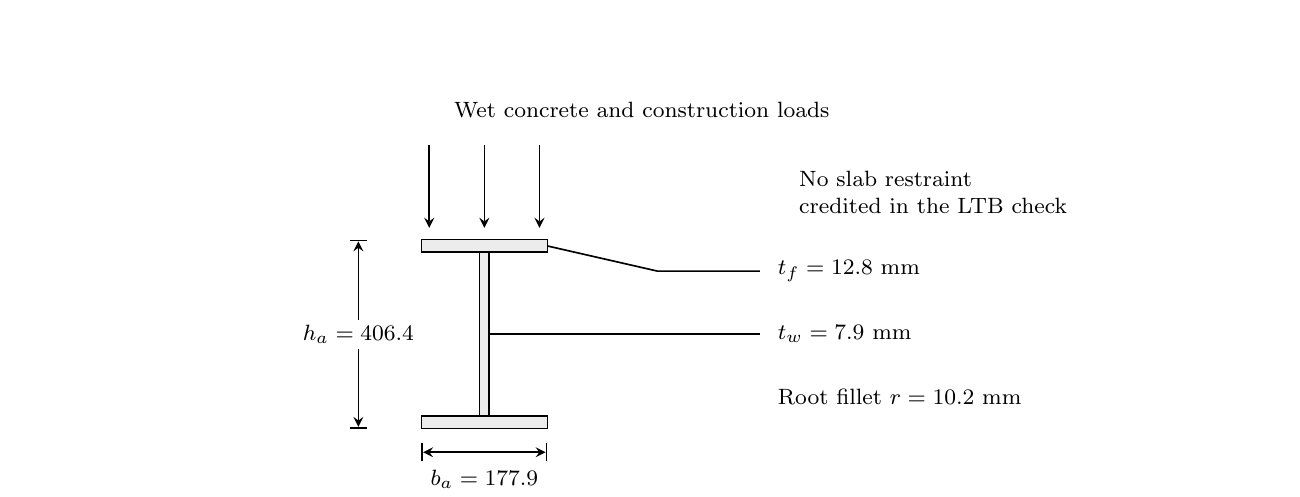
\begin{tikzpicture}[x=1cm,y=1cm,line width=.6pt,>=stealth,font=\fontsize{8.5}{10}\selectfont]\path[use as bounding box] (0,0) rectangle (15.8,5.6);\draw[fill=gray!15] (5,1) rectangle ++(1.6,.16);\draw[fill=gray!15] (5.74,1.16) rectangle ++(.12,2.08);\draw[fill=gray!15] (5,3.24) rectangle ++(1.6,.16);\foreach \x in {5.1,5.8,6.5}{\draw[->] (\x,4.6)--(\x,3.55);}\node at (7.8,5.05){Wet concrete and construction loads};\node[align=left] at (11.5,4){No slab restraint\\credited in the LTB check};\draw[|<->|] (4.2,1)--(4.2,3.4) node[midway,fill=white,inner sep=2pt]{$h_a=406.4$};\draw[|<->|] (5,0.7)--(6.6,0.7) node[midway,below=3pt]{$b_a=177.9$};\draw (6.6,3.32)--(8,3)--(9.3,3);\node[anchor=west] at (9.4,3){$t_f=12.8$ mm};\draw (5.86,2.2)--(8,2.2)--(9.3,2.2);\node[anchor=west] at (9.4,2.2){$t_w=7.9$ mm};\node[anchor=west] at (9.4,1.4){Root fillet $r=10.2$ mm};\node at (7.9,-.15){Dimensions in mm; section schematic; fillets omitted.};\end{tikzpicture}\end{minipage}\par\vspace{5pt}

\sect{6. EFFECTIVE SLAB WIDTH}
{\small\color{muted}EC4 §5.4.1.2: simply supported midspan Le = L; one stud row, b0 = 0.}\par
\Needspace{24mm}\begin{minipage}{\linewidth}{\small\bfseries\color{muted}Equivalent span}\par\vspace{3pt}{\small\eq{L_e\coloneq  L}\par\vspace{2pt}\eq{=8\,\mathrm{m}}\par\vspace{2pt}\eq{\color{navy}=8\,\mathrm{m}}}\par\vspace{7pt}\end{minipage}\par
\Needspace{24mm}\begin{minipage}{\linewidth}{\small\bfseries\color{muted}Available width each side}\par\vspace{3pt}{\small\eq{b_1\coloneq  \frac{s_b-b_0}{2}}\par\vspace{2pt}\eq{=\frac{3\,\mathrm{m}-0\,\mathrm{m}}{2}}\par\vspace{2pt}\eq{\color{navy}=1500\,\mathrm{mm}}}\par\vspace{7pt}\end{minipage}\par
\Needspace{24mm}\begin{minipage}{\linewidth}{\small\bfseries\color{muted}Effective width each side}\par\vspace{3pt}{\small\eq{b_e\coloneq  \min(\frac{L_e}{8},b_1)}\par\vspace{2pt}\eq{=\min(\frac{8\,\mathrm{m}}{8},1.5\,\mathrm{m})}\par\vspace{2pt}\eq{\color{navy}=1000\,\mathrm{mm}}}\par\vspace{7pt}\end{minipage}\par
\Needspace{24mm}\begin{minipage}{\linewidth}{\small\bfseries\color{muted}Effective width at midspan}\par\vspace{3pt}{\small\eq{b_{eff}\coloneq  b_0+2b_e}\par\vspace{2pt}\eq{=0\,\mathrm{m}+2\cdot (1\,\mathrm{m})}\par\vspace{2pt}\eq{\color{navy}=2000\,\mathrm{mm}}}\par\vspace{7pt}\end{minipage}\par

\Needspace{65mm}\begin{minipage}{\linewidth}\vspace{4pt}{\bfseries\color{navy}D03 — Midspan effective width; not the 3 m tributary load width}\par

\centering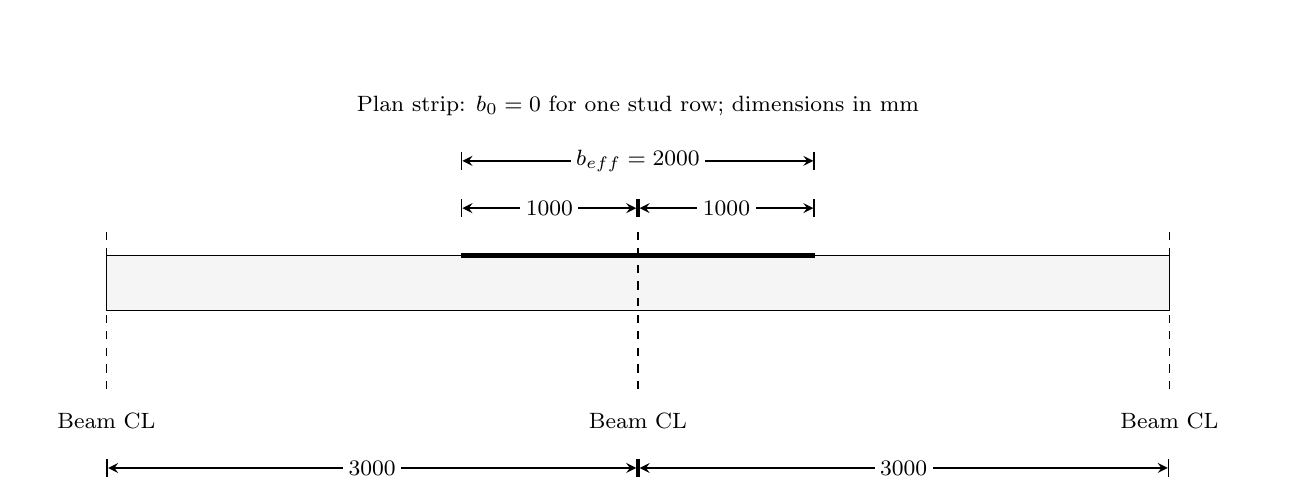
\begin{tikzpicture}[x=1cm,y=1cm,line width=.6pt,>=stealth,font=\fontsize{8.5}{10}\selectfont]\path[use as bounding box] (0,0) rectangle (15.8,5.6);\draw[fill=gray!8] (1,2.5) rectangle (14.5,3.2);\foreach \x in {1,7.75,14.5}{\draw[dashed] (\x,1.5)--(\x,3.6);\node at (\x,1.1){Beam CL};}\draw[line width=2pt] (5.5,3.2)--(10,3.2);\draw[|<->|] (5.5,4.4)--(10,4.4) node[midway,fill=white,inner sep=2pt]{$b_{eff}=2000$};\draw[|<->|] (1,0.5)--(7.75,0.5) node[midway,fill=white,inner sep=2pt]{3000};\draw[|<->|] (7.75,0.5)--(14.5,0.5) node[midway,fill=white,inner sep=2pt]{3000};\draw[|<->|] (5.5,3.8)--(7.75,3.8) node[midway,fill=white,inner sep=2pt]{1000};\draw[|<->|] (7.75,3.8)--(10,3.8) node[midway,fill=white,inner sep=2pt]{1000};\node at (7.75,5.1){Plan strip: $b_0=0$ for one stud row; dimensions in mm};\end{tikzpicture}\end{minipage}\par\vspace{5pt}

\sect{7. SHEAR CONNECTOR RESISTANCE}
\Needspace{25mm}\begin{longtable}{@{}p{0.53\linewidth}p{0.43\linewidth}@{}}\rowcolor{light}\textbf{Parameter / reference} & \textbf{Definition / value}\\\midrule
{\small Headed stud shank diameter} & {\small $d_{sc}\coloneq 19\,\mathrm{mm}$}\\[5pt]
{\small Stud height after welding} & {\small $h_{sc}\coloneq 100\,\mathrm{mm}$}\\[5pt]
{\small Stud ultimate strength, <= 500 MPa} & {\small $f_u\coloneq 450\,\mathrm{MPa}$}\\[5pt]
{\small Studs in each half-span, single row} & {\small $n_h\coloneq 24$}\\[5pt]\bottomrule\end{longtable}\Needspace{24mm}\begin{minipage}{\linewidth}{\small\bfseries\color{muted}Longitudinal pitch: first/last centres at half pitch}\par\vspace{3pt}{\small\eq{s_{sc}\coloneq  \frac{L}{2n_h}}\par\vspace{2pt}\eq{=\frac{8\,\mathrm{m}}{2\cdot 24}}\par\vspace{2pt}\eq{\color{navy}=166.667\,\mathrm{mm}}}\par\vspace{7pt}\end{minipage}\par
\Needspace{24mm}\begin{minipage}{\linewidth}{\small\bfseries\color{muted}EC4 §6.6.3.1, hsc/d >= 4 here}\par\vspace{3pt}{\small\eq{\alpha_{sc}\coloneq  \min(1,0.2(\frac{h_{sc}}{d_{sc}}+1))}\par\vspace{2pt}\eq{=\min(1,0.2(\frac{0.1\,\mathrm{m}}{0.019\,\mathrm{m}}+1))}\par\vspace{2pt}\eq{\color{navy}=1}}\par\vspace{7pt}\end{minipage}\par
\Needspace{24mm}\begin{minipage}{\linewidth}{\small\bfseries\color{muted}EC4 (6.18): stud steel failure}\par\vspace{3pt}{\small\eq{P_{s.Rd}\coloneq  \frac{0.8 f_u \pi d_{sc}^2}{4\gamma_V}}\par\vspace{2pt}\eq{=\frac{0.8\cdot (450\,\mathrm{MPa})\pi(0.019\,\mathrm{m})^{2}}{4\cdot 1.25}}\par\vspace{2pt}\eq{\color{navy}=81.656\,\mathrm{kN}}}\par\vspace{7pt}\end{minipage}\par
\Needspace{24mm}\begin{minipage}{\linewidth}{\small\bfseries\color{muted}EC4 (6.19): concrete failure}\par\vspace{3pt}{\small\eq{P_{c.Rd}\coloneq  \frac{0.29\alpha_{sc}d_{sc}^2\sqrt{f_{ck}E_{cm}}}{\gamma_V}}\par\vspace{2pt}\eq{=\frac{0.29\cdot 1(0.019\,\mathrm{m})^{2}\sqrt{(30\,\mathrm{MPa})\cdot (33000\,\mathrm{MPa})}}{1.25}}\par\vspace{2pt}\eq{\color{navy}=83.332\,\mathrm{kN}}}\par\vspace{7pt}\end{minipage}\par
\Needspace{25mm}\begin{longtable}{@{}p{0.53\linewidth}p{0.43\linewidth}@{}}\rowcolor{light}{\small Stud material limit, EC4 §6.6.3.1} & {\small $f_{u}=450\,\mathrm{MPa}\;\le\;500\,\mathrm{MPa}\quad\text{\color{pass}PASS}$}\\[5pt]\end{longtable}\Needspace{24mm}\begin{minipage}{\linewidth}{\small\bfseries\color{muted}Solid slab stud design resistance}\par\vspace{3pt}{\small\eq{P_{Rd}\coloneq  \min(P_{s.Rd},P_{c.Rd})}\par\vspace{2pt}\eq{=\min(81.656\,\mathrm{kN},83.332\,\mathrm{kN})}\par\vspace{2pt}\eq{\color{navy}=81.656\,\mathrm{kN}}}\par\vspace{7pt}\end{minipage}\par
\Needspace{25mm}\begin{longtable}{@{}p{0.53\linewidth}p{0.43\linewidth}@{}}\rowcolor{light}\textbf{Parameter / reference} & \textbf{Definition / value}\\\midrule
{\small Ductile stud geometry, EC4 §6.6.1.2} & {\small $4d_{\mathrm{sc}}=0.076\,\mathrm{m}\;\le\;h_{\mathrm{sc}}=0.1\,\mathrm{m}\quad\text{\color{pass}PASS}$}\\[5pt]
{\small Diameter range, lower bound} & {\small $16\mathrm{mm}=0.016\,\mathrm{m}\;\le\;d_{\mathrm{sc}}=0.019\,\mathrm{m}\quad\text{\color{pass}PASS}$}\\[5pt]
{\small Diameter range, upper bound} & {\small $d_{\mathrm{sc}}=0.019\,\mathrm{m}\;\le\;0.025\,\mathrm{m}\quad\text{\color{pass}PASS}$}\\[5pt]
{\small EC4 §6.6.5.7: minimum longitudinal spacing} & {\small $5d_{\mathrm{sc}}=0.095\,\mathrm{m}\;\le\;s_{\mathrm{sc}}=0.1667\,\mathrm{m}\quad\text{\color{pass}PASS}$}\\[5pt]
{\small Maximum longitudinal spacing, buildings} & {\small $s_{\mathrm{sc}}=0.1667\,\mathrm{m}\;\le\;\min\left(6h_{c},800\mathrm{mm}\right)=0.8\,\mathrm{m}\quad\text{\color{pass}PASS}$}\\[5pt]\bottomrule\end{longtable}\Needspace{24mm}\begin{minipage}{\linewidth}{\small\bfseries\color{muted}Slab cover above stud head}\par\vspace{3pt}{\small\eq{c_{sc}\coloneq  h_c-h_{sc}}\par\vspace{2pt}\eq{=0.15\,\mathrm{m}-0.1\,\mathrm{m}}\par\vspace{2pt}\eq{\color{navy}=50\,\mathrm{mm}}}\par\vspace{7pt}\end{minipage}\par
\Needspace{25mm}\begin{longtable}{@{}p{0.53\linewidth}p{0.43\linewidth}@{}}\rowcolor{light}{\small Nominal top cover >= 20 mm, EC4 §6.6.5.2} & {\small $20\mathrm{mm}=0.02\,\mathrm{m}\;\le\;c_{\mathrm{sc}}=0.05\,\mathrm{m}\quad\text{\color{pass}PASS}$}\\[5pt]\end{longtable}\Needspace{24mm}\begin{minipage}{\linewidth}{\small\bfseries\color{muted}Stud shank edge to steel flange edge}\par\vspace{3pt}{\small\eq{e_{sc}\coloneq  \frac{b_a-d_{sc}}{2}}\par\vspace{2pt}\eq{=\frac{0.1779\,\mathrm{m}-0.019\,\mathrm{m}}{2}}\par\vspace{2pt}\eq{\color{navy}=79.45\,\mathrm{mm}}}\par\vspace{7pt}\end{minipage}\par
\Needspace{25mm}\begin{longtable}{@{}p{0.53\linewidth}p{0.43\linewidth}@{}}\rowcolor{light}{\small EC4 §6.6.5.6: steel flange edge >= 20 mm} & {\small $20\mathrm{mm}=0.02\,\mathrm{m}\;\le\;e_{\mathrm{sc}}=0.07945\,\mathrm{m}\quad\text{\color{pass}PASS}$}\\[5pt]\end{longtable}
{\small\color{muted}Single row: transverse stud pitch is inapplicable. Weld and head dimensions require specification.}\par
\Needspace{65mm}\begin{minipage}{\linewidth}\vspace{4pt}{\bfseries\color{navy}D09 — Single stud row: 48 total; 24 per half-span}\par

\centering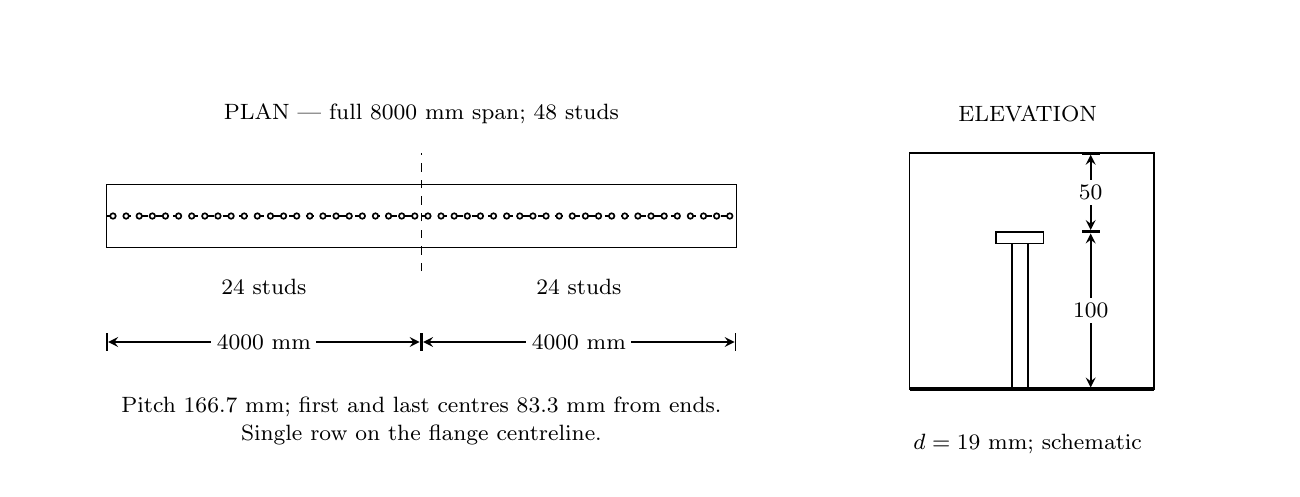
\begin{tikzpicture}[x=1cm,y=1cm,line width=.6pt,>=stealth,font=\fontsize{8.5}{10}\selectfont]\path[use as bounding box] (0,0) rectangle (15.8,5.6);\node at (5,5){PLAN — full 8000 mm span; 48 studs};\draw (1,3.3) rectangle (9,4.1);\draw[dashed] (1,3.7)--(9,3.7);\foreach \i in {0,...,47}{\pgfmathsetmacro{\x}{1+(\i+.5)/6}\draw[fill=white] (\x,3.7) circle (.035);}\draw[dashed] (5,3)--(5,4.5);\node at (3,2.8){24 studs};\node at (7,2.8){24 studs};\draw[|<->|] (1,2.1)--(5,2.1) node[midway,fill=white,inner sep=2pt]{4000 mm};\draw[|<->|] (5,2.1)--(9,2.1) node[midway,fill=white,inner sep=2pt]{4000 mm};\node[align=center] at (5,1.1){Pitch 166.7 mm; first and last centres 83.3 mm from ends.\\Single row on the flange centreline.};\draw (11.2,1.5) rectangle (14.3,4.5);\draw[line width=1.3pt] (11.2,1.5)--(14.3,1.5);\draw (12.5,1.5) rectangle (12.7,3.35);\draw (12.3,3.35) rectangle (12.9,3.5);\draw[|<->|] (13.5,1.5)--(13.5,3.5) node[midway,fill=white,inner sep=2pt]{100};\draw[|<->|] (13.5,3.5)--(13.5,4.5) node[midway,fill=white,inner sep=2pt]{50};\node at (12.7,5){ELEVATION};\node at (12.7,.8){$d=19$ mm; schematic};\end{tikzpicture}\end{minipage}\par\vspace{5pt}

\sect{8. DEGREE OF SHEAR CONNECTION}
\Needspace{24mm}\begin{minipage}{\linewidth}{\small\bfseries\color{muted}Maximum slab compression, EC4 §6.2.1.2}\par\vspace{3pt}{\small\eq{N_{c.Rd}\coloneq  0.85 f_{cd}b_{eff}h_c}\par\vspace{2pt}\eq{=0.85\cdot (20\,\mathrm{MPa})\cdot (2\,\mathrm{m})\cdot (0.15\,\mathrm{m})}\par\vspace{2pt}\eq{\color{navy}=5100\,\mathrm{kN}}}\par\vspace{7pt}\end{minipage}\par
\Needspace{24mm}\begin{minipage}{\linewidth}{\small\bfseries\color{muted}Steel tensile resistance}\par\vspace{3pt}{\small\eq{N_{a.Rd}\coloneq  A_a f_{yd}}\par\vspace{2pt}\eq{=(7650\,\mathrm{mm}^{2})\cdot (355\,\mathrm{MPa})}\par\vspace{2pt}\eq{\color{navy}=2715.75\,\mathrm{kN}}}\par\vspace{7pt}\end{minipage}\par
\Needspace{24mm}\begin{minipage}{\linewidth}{\small\bfseries\color{muted}Force needed for full connection, EC4 §6.6.2}\par\vspace{3pt}{\small\eq{N_{c.f}\coloneq  \min(N_{c.Rd},N_{a.Rd})}\par\vspace{2pt}\eq{=\min(5100\,\mathrm{kN},2715.75\,\mathrm{kN})}\par\vspace{2pt}\eq{\color{navy}=2715.75\,\mathrm{kN}}}\par\vspace{7pt}\end{minipage}\par
\Needspace{24mm}\begin{minipage}{\linewidth}{\small\bfseries\color{muted}Available transfer per half-span}\par\vspace{3pt}{\small\eq{N_{conn}\coloneq  n_h P_{Rd}}\par\vspace{2pt}\eq{=24\cdot (81.656\,\mathrm{kN})}\par\vspace{2pt}\eq{\color{navy}=1959.751\,\mathrm{kN}}}\par\vspace{7pt}\end{minipage}\par
\Needspace{24mm}\begin{minipage}{\linewidth}{\small\bfseries\color{muted}Degree of connection: not a utilisation ratio}\par\vspace{3pt}{\small\eq{\eta\coloneq  \min(1,\frac{N_{conn}}{N_{c.f}})}\par\vspace{2pt}\eq{=\min(1,\frac{1959.751\,\mathrm{kN}}{2715.75\,\mathrm{kN}})}\par\vspace{2pt}\eq{\color{navy}=0.7216}}\par\vspace{7pt}\end{minipage}\par
\Needspace{24mm}\begin{minipage}{\linewidth}{\small\bfseries\color{muted}EC4 §6.6.1.2(1), equal flanges, Le <= 25 m}\par\vspace{3pt}{\small\eq{\eta_{min}\coloneq  \max(0.4,1-\frac{355\,\mathrm{MPa}}{f_y}(0.75-0.03\frac{L_e}{1\,\mathrm{m}}))}\par\vspace{2pt}\eq{=\max(0.4,1-\frac{355\mathrm{MPa}}{355\,\mathrm{MPa}}(0.75-0.03\frac{8\,\mathrm{m}}{1\mathrm{m}}))}\par\vspace{2pt}\eq{\color{navy}=0.49}}\par\vspace{7pt}\end{minipage}\par
\Needspace{25mm}\begin{longtable}{@{}p{0.53\linewidth}p{0.43\linewidth}@{}}\rowcolor{light}\textbf{Parameter / reference} & \textbf{Definition / value}\\\midrule
{\small Minimum connection degree} & {\small $\eta_{\mathrm{min}}=0.49\;\le\;\eta=0.7216\quad\text{\color{pass}PASS}$}\\[5pt]
{\small Branch applicability} & {\small $L_{e}=8\,\mathrm{m}\;\le\;25\,\mathrm{m}\quad\text{\color{pass}PASS}$}\\[5pt]\bottomrule\end{longtable}\Needspace{24mm}\begin{minipage}{\linewidth}{\small\bfseries\color{muted}Concrete force available at resistance}\par\vspace{3pt}{\small\eq{N_c\coloneq  \min(N_{conn},N_{c.f})}\par\vspace{2pt}\eq{=\min(1959.751\,\mathrm{kN},2715.75\,\mathrm{kN})}\par\vspace{2pt}\eq{\color{navy}=1959.751\,\mathrm{kN}}}\par\vspace{7pt}\end{minipage}\par

\sect{9. COMPOSITE BENDING RESISTANCE}
{\small\color{muted}EC4 §6.2.1.2 / §6.2.1.3: Class 1/2, ductile studs and verified minimum connection.}\par
{\small\color{muted}Use the conservative linear interaction method, §6.2.1.3(3), not an invented eta multiplier.}\par
\Needspace{24mm}\begin{minipage}{\linewidth}{\small\bfseries\color{muted}Full-connection slab compression depth}\par\vspace{3pt}{\small\eq{x_f\coloneq  \frac{N_{c.f}}{0.85 f_{cd}b_{eff}}}\par\vspace{2pt}\eq{=\frac{2715.75\,\mathrm{kN}}{0.85\cdot (20\,\mathrm{MPa})\cdot (2\,\mathrm{m})}}\par\vspace{2pt}\eq{\color{navy}=79.875\,\mathrm{mm}}}\par\vspace{7pt}\end{minipage}\par
\Needspace{25mm}\begin{longtable}{@{}p{0.53\linewidth}p{0.43\linewidth}@{}}\rowcolor{light}{\small Full-connection PNA is within slab in this example} & {\small $x_{f}=0.07988\,\mathrm{m}\;\le\;h_{c}=0.15\,\mathrm{m}\quad\text{\color{pass}PASS}$}\\[5pt]\end{longtable}\Needspace{24mm}\begin{minipage}{\linewidth}{\small\bfseries\color{muted}Full-connection lever arm}\par\vspace{3pt}{\small\eq{z_f\coloneq  h_c+\frac{h_a}{2}-\frac{x_f}{2}}\par\vspace{2pt}\eq{=0.15\,\mathrm{m}+\frac{0.4064\,\mathrm{m}}{2}-\frac{0.07988\,\mathrm{m}}{2}}\par\vspace{2pt}\eq{\color{navy}=313.262\,\mathrm{mm}}}\par\vspace{7pt}\end{minipage}\par
\Needspace{24mm}\begin{minipage}{\linewidth}{\small\bfseries\color{muted}Full-connection resistance: slab PNA branch only}\par\vspace{3pt}{\small\eq{M_{pl.Rd}\coloneq  N_{c.f}z_f}\par\vspace{2pt}\eq{=(2715.75\,\mathrm{kN})\cdot (0.3133\,\mathrm{m})}\par\vspace{2pt}\eq{\color{navy}=850.743\,\mathrm{kN}\cdot \mathrm{m}}}\par\vspace{7pt}\end{minipage}\par
\Needspace{24mm}\begin{minipage}{\linewidth}{\small\bfseries\color{muted}Conservative partial resistance, EC4 §6.2.1.3(3)}\par\vspace{3pt}{\small\eq{M_{Rd}\coloneq  M_{a.Rd}+\eta(M_{pl.Rd}-M_{a.Rd})}\par\vspace{2pt}\eq{=426\,\mathrm{kN}\cdot \mathrm{m}+0.7216(850.743\,\mathrm{kN}\cdot \mathrm{m}-426\,\mathrm{kN}\cdot \mathrm{m})}\par\vspace{2pt}\eq{\color{navy}=732.505\,\mathrm{kN}\cdot \mathrm{m}}}\par\vspace{7pt}\end{minipage}\par
\Needspace{24mm}\begin{minipage}{\linewidth}{\small\bfseries\color{muted}Final composite bending}\par\vspace{3pt}{\small\eq{\mathrm{UR}_{M.2}\coloneq  \frac{M_{2.Ed}}{M_{Rd}}}\par\vspace{2pt}\eq{=\frac{284.467\,\mathrm{kN}\cdot \mathrm{m}}{732.505\,\mathrm{kN}\cdot \mathrm{m}}}\par\vspace{2pt}\eq{\color{navy}=0.3883}}\par\vspace{7pt}\end{minipage}\par
\Needspace{25mm}\begin{longtable}{@{}p{0.53\linewidth}p{0.43\linewidth}@{}}\rowcolor{light}{\small Acceptance} & {\small $\mathrm{UR}_{\mathrm{M.2}}=0.3883\;\le\;1\quad\text{\color{pass}PASS}$}\\[5pt]\end{longtable}\Needspace{24mm}\begin{minipage}{\linewidth}{\small\bfseries\color{muted}Uniform stud distribution applicability, §6.6.1.3}\par\vspace{3pt}{\small\eq{r_M\coloneq  \frac{M_{pl.Rd}}{M_{a.Rd}}}\par\vspace{2pt}\eq{=\frac{850.743\,\mathrm{kN}\cdot \mathrm{m}}{426\,\mathrm{kN}\cdot \mathrm{m}}}\par\vspace{2pt}\eq{\color{navy}=1.997}}\par\vspace{7pt}\end{minipage}\par
\Needspace{25mm}\begin{longtable}{@{}p{0.53\linewidth}p{0.43\linewidth}@{}}\rowcolor{light}{\small Uniform spacing resistance ratio limit} & {\small $r_{M}=1.997\;\le\;2.5\quad\text{\color{pass}PASS}$}\\[5pt]\end{longtable}
{\small\color{muted}For UDL the moment envelope and connector distribution must also remain compatible.}\par
\Needspace{24mm}\begin{minipage}{\linewidth}{\small\bfseries\color{muted}At partial resistance: slab compression depth}\par\vspace{3pt}{\small\eq{x_c\coloneq  \frac{N_c}{0.85 f_{cd}b_{eff}}}\par\vspace{2pt}\eq{=\frac{1959.751\,\mathrm{kN}}{0.85\cdot (20\,\mathrm{MPa})\cdot (2\,\mathrm{m})}}\par\vspace{2pt}\eq{\color{navy}=57.64\,\mathrm{mm}}}\par\vspace{7pt}\end{minipage}\par
\Needspace{24mm}\begin{minipage}{\linewidth}{\small\bfseries\color{muted}Required compressed steel area from equilibrium}\par\vspace{3pt}{\small\eq{A_{ac}\coloneq  \frac{A_a-N_c/f_{yd}}{2}}\par\vspace{2pt}\eq{=\frac{7650\,\mathrm{mm}^{2}-1959.751\,\mathrm{kN}/(355\,\mathrm{MPa})}{2}}\par\vspace{2pt}\eq{\color{navy}=1064.788\,\mathrm{mm}^{2}}}\par\vspace{7pt}\end{minipage}\par
\Needspace{24mm}\begin{minipage}{\linewidth}{\small\bfseries\color{muted}Steel area above top-flange underside}\par\vspace{3pt}{\small\eq{A_f\coloneq  b_a t_f}\par\vspace{2pt}\eq{=(0.1779\,\mathrm{m})\cdot (0.0128\,\mathrm{m})}\par\vspace{2pt}\eq{\color{navy}=2277.12\,\mathrm{mm}^{2}}}\par\vspace{7pt}\end{minipage}\par
\Needspace{25mm}\begin{longtable}{@{}p{0.53\linewidth}p{0.43\linewidth}@{}}\rowcolor{light}{\small Example steel PNA lies in top flange} & {\small $A_{\mathrm{ac}}=1064.788\,\mathrm{mm}^{2}\;\le\;A_{f}=2277.12\,\mathrm{mm}^{2}\quad\text{\color{pass}PASS}$}\\[5pt]\end{longtable}\Needspace{24mm}\begin{minipage}{\linewidth}{\small\bfseries\color{muted}Steel PNA below steel top, flange branch}\par\vspace{3pt}{\small\eq{y_a\coloneq  \frac{A_{ac}}{b_a}}\par\vspace{2pt}\eq{=\frac{1064.788\,\mathrm{mm}^{2}}{0.1779\,\mathrm{m}}}\par\vspace{2pt}\eq{\color{navy}=5.985\,\mathrm{mm}}}\par\vspace{7pt}\end{minipage}\par
\Needspace{24mm}\begin{minipage}{\linewidth}{\small\bfseries\color{muted}Compression resultant in steel}\par\vspace{3pt}{\small\eq{C_a\coloneq  A_{ac}f_{yd}}\par\vspace{2pt}\eq{=(1064.788\,\mathrm{mm}^{2})\cdot (355\,\mathrm{MPa})}\par\vspace{2pt}\eq{\color{navy}=378\,\mathrm{kN}}}\par\vspace{7pt}\end{minipage}\par
\Needspace{24mm}\begin{minipage}{\linewidth}{\small\bfseries\color{muted}Tension resultant in steel}\par\vspace{3pt}{\small\eq{T_a\coloneq  (A_a-A_{ac})f_{yd}}\par\vspace{2pt}\eq{=(7650\,\mathrm{mm}^{2}-1064.788\,\mathrm{mm}^{2})\cdot (355\,\mathrm{MPa})}\par\vspace{2pt}\eq{\color{navy}=2337.75\,\mathrm{kN}}}\par\vspace{7pt}\end{minipage}\par
\Needspace{24mm}\begin{minipage}{\linewidth}{\small\bfseries\color{muted}Force equilibrium residual}\par\vspace{3pt}{\small\eq{R_N\coloneq  C_a+N_c-T_a}\par\vspace{2pt}\eq{=378\,\mathrm{kN}+1959.751\,\mathrm{kN}-2337.75\,\mathrm{kN}}\par\vspace{2pt}\eq{\color{navy}=0\,\mathrm{kN}}}\par\vspace{7pt}\end{minipage}\par
\Needspace{24mm}\begin{minipage}{\linewidth}{\small\bfseries\color{muted}Direct plastic stress-block resistance, top-flange PNA branch}\par\vspace{3pt}{\small\eq{M_{direct}\coloneq  f_{yd}A_a(h_c+\frac{h_a}{2})-2f_{yd}A_{ac}(h_c+\frac{y_a}{2})-\frac{N_c x_c}{2}}\par\vspace{2pt}\eq{=(355\,\mathrm{MPa})\cdot (7650\,\mathrm{mm}^{2})\cdot (0.15\,\mathrm{m}+\frac{0.4064\,\mathrm{m}}{2})-2\cdot (355\,\mathrm{MPa})(1064.788\,\mathrm{mm}^{2})\cdot (0.15\,\mathrm{m}+\frac{0.005985\,\mathrm{m}}{2})-\frac{(1959.751\,\mathrm{kN})\cdot (0.05764\,\mathrm{m})}{2}}\par\vspace{2pt}\eq{\color{navy}=787.061\,\mathrm{kN}\cdot \mathrm{m}}}\par\vspace{7pt}\end{minipage}\par
\Needspace{24mm}\begin{minipage}{\linewidth}{\small\bfseries\color{muted}Conservative linear result below direct plastic result}\par\vspace{3pt}{\small\eq{M_{\mathrm{Rd}}=732.505\,\mathrm{kN}\cdot \mathrm{m}\;\le\;M_{\mathrm{direct}}=787.061\,\mathrm{kN}\cdot \mathrm{m}\quad\text{\color{pass}PASS}}}\par\vspace{7pt}\end{minipage}\par

{\small\color{muted}Partial interaction permits distinct slab and steel neutral axes; do not join them into one PNA.}\par
{\small\color{muted}General PNA solution and admissibility are set out in the linked annex.}\par
\Needspace{65mm}\begin{minipage}{\linewidth}\vspace{4pt}{\bfseries\color{navy}D05 — Full connection: slab PNA; steel entirely in tension}\par

\centering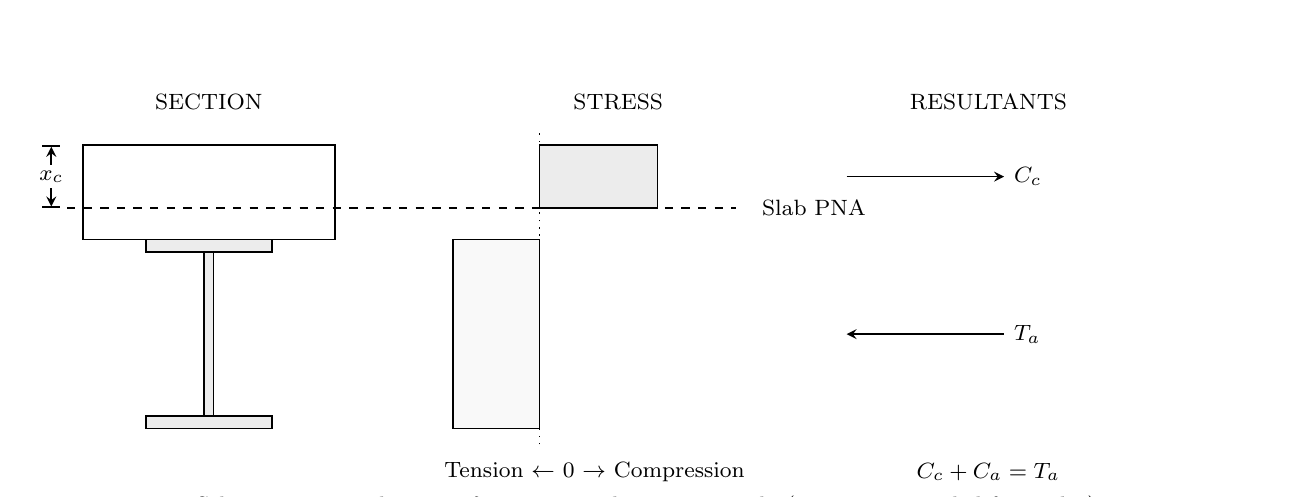
\begin{tikzpicture}[x=1cm,y=1cm,line width=.6pt,>=stealth,font=\fontsize{8.5}{10}\selectfont]\path[use as bounding box] (0,0) rectangle (15.8,5.6);\draw[fill=gray!15] (1.5,1) rectangle ++(1.6,.16);\draw[fill=gray!15] (2.24,1.16) rectangle ++(.12,2.08);\draw[fill=gray!15] (1.5,3.24) rectangle ++(1.6,.16);\draw (0.7,3.4) rectangle (3.9,4.6);\node at (2.3,5.15){SECTION};\node at (7.5,5.15){STRESS};\node at (12.2,5.15){RESULTANTS};\draw[dashed] (.5,3.8)--(9,3.8);\node[anchor=west] at (9.2,3.8){Slab PNA};\draw[dotted] (6.5,.8)--(6.5,4.8);\draw[fill=gray!15] (6.5,3.8) rectangle (8,4.6);\draw[->] (10.4,4.199999999999999)--(12.4,4.199999999999999) node[right]{$C_c$};\draw[fill=gray!5] (5.4,1) rectangle (6.5,3.4);\draw[<-] (10.4,2.2)--(12.4,2.2) node[right]{$T_a$};\node at (7.2,.45){Tension $\leftarrow$ 0 $\rightarrow$ Compression};\node at (12.2,.45){$C_c+C_a=T_a$};\draw[|<->|] (0.3,3.8)--(0.3,4.6) node[midway,fill=white,inner sep=2pt]{$x_c$};\node at (7.9,0){Schematic stress diagram; force arrows shown separately (not an area-scaled force plot).};\end{tikzpicture}\end{minipage}\par\vspace{5pt}

{\small\color{navy}Annex: General plastic equilibrium and PNA branches}\par
\sect{10. VERTICAL SHEAR AND INTERACTION}
\Needspace{24mm}\begin{minipage}{\linewidth}{\small\bfseries\color{muted}Final vertical shear: steel web only}\par\vspace{3pt}{\small\eq{\mathrm{UR}_{V.2}\coloneq  \frac{V_{2.Ed}}{V_{pl.Rd}}}\par\vspace{2pt}\eq{=\frac{142.234\,\mathrm{kN}}{708.749\,\mathrm{kN}}}\par\vspace{2pt}\eq{\color{navy}=0.2007}}\par\vspace{7pt}\end{minipage}\par
\Needspace{25mm}\begin{longtable}{@{}p{0.53\linewidth}p{0.43\linewidth}@{}}\rowcolor{light}\textbf{Parameter / reference} & \textbf{Definition / value}\\\midrule
{\small Acceptance} & {\small $\mathrm{UR}_{\mathrm{V.2}}=0.2007\;\le\;1\quad\text{\color{pass}PASS}$}\\[5pt]
{\small EC4 §6.2.2.4: low-shear branch used} & {\small $V_{\mathrm{2.Ed}}=142.234\,\mathrm{kN}\;\le\;0.5V_{\mathrm{pl.Rd}}=354.375\,\mathrm{kN}\quad\text{\color{pass}PASS}$}\\[5pt]\bottomrule\end{longtable}\Needspace{24mm}\begin{minipage}{\linewidth}{\small\bfseries\color{muted}Shear buckling slenderness, EC3 §6.2.6(6)}\par\vspace{3pt}{\small\eq{\lambda_w\coloneq  \frac{h_a-2t_f}{t_w}}\par\vspace{2pt}\eq{=\frac{0.4064\,\mathrm{m}-2\cdot (0.0128\,\mathrm{m})}{0.0079\,\mathrm{m}}}\par\vspace{2pt}\eq{\color{navy}=48.203}}\par\vspace{7pt}\end{minipage}\par
\Needspace{25mm}\begin{longtable}{@{}p{0.53\linewidth}p{0.43\linewidth}@{}}\rowcolor{light}{\small No shear buckling needed, eta = 1.2 recommended} & {\small $\lambda_{w}=48.203\;\le\;\frac{72\varepsilon}{1.2}=48.817\quad\text{\color{pass}PASS}$}\\[5pt]\end{longtable}
{\small\color{muted}If either limit fails, this worksheet branch is inapplicable: perform reduced M-V resistance.}\par
\sect{11. LONGITUDINAL SHEAR AND REINFORCEMENT}
{\small\color{muted}EC4 §6.6.6; EC2 §6.2.4. Symmetric internal beam, two vertical shear planes beside studs.}\par
{\small\color{muted}Design for connector resistance envelope; half the transfer to each slab outstand.}\par
\Needspace{24mm}\begin{minipage}{\linewidth}{\small\bfseries\color{muted}Conservative peak local transfer, two times uniform resistance flow}\par\vspace{3pt}{\small\eq{v_{L.Ed}\coloneq  \frac{2N_c}{L h_c}}\par\vspace{2pt}\eq{=\frac{2\cdot (1959.751\,\mathrm{kN})}{(8\,\mathrm{m})\cdot (0.15\,\mathrm{m})}}\par\vspace{2pt}\eq{\color{navy}=3.266\,\mathrm{MPa}}}\par\vspace{7pt}\end{minipage}\par
\Needspace{25mm}\begin{longtable}{@{}p{0.53\linewidth}p{0.43\linewidth}@{}}\rowcolor{light}\textbf{Parameter / reference} & \textbf{Definition / value}\\\midrule
{\small Compression strut cotangent, EC2 1 <= cot theta <= 2} & {\small $c_{theta}\coloneq 2$}\\[5pt]
{\small Transverse reinforcement per plane, one continuous layer} & {\small $d_s\coloneq 10\,\mathrm{mm}$}\\[5pt]
{\small Bar spacing along beam} & {\small $s_f\coloneq 150\,\mathrm{mm}$}\\[5pt]\bottomrule\end{longtable}\Needspace{24mm}\begin{minipage}{\linewidth}{\small\bfseries\color{muted}Required transverse steel per unit beam length, EC2 (6.21)}\par\vspace{3pt}{\small\eq{a_{sf.req}\coloneq  \frac{v_{L.Ed} h_c}{f_{sd}c_{theta}}}\par\vspace{2pt}\eq{=\frac{(3.266\,\mathrm{MPa})\cdot (0.15\,\mathrm{m})}{(434.783\,\mathrm{MPa})\cdot 2}}\par\vspace{2pt}\eq{\color{navy}=563.428\,\mathrm{mm}^{2}/\mathrm{m}}}\par\vspace{7pt}\end{minipage}\par
\Needspace{24mm}\begin{minipage}{\linewidth}{\small\bfseries\color{muted}Provided steel crossing each shear plane}\par\vspace{3pt}{\small\eq{a_{sf}\coloneq  \frac{\pi d_s^2}{4s_f}}\par\vspace{2pt}\eq{=\frac{\pi(0.01\,\mathrm{m})^{2}}{4\cdot (0.15\,\mathrm{m})}}\par\vspace{2pt}\eq{\color{navy}=523.599\,\mathrm{mm}^{2}/\mathrm{m}}}\par\vspace{7pt}\end{minipage}\par
\Needspace{24mm}\begin{minipage}{\linewidth}{\small\bfseries\color{muted}Transverse reinforcement}\par\vspace{3pt}{\small\eq{\mathrm{UR}_{sf}\coloneq  \frac{a_{sf.req}}{a_{sf}}}\par\vspace{2pt}\eq{=\frac{0.0005634\,\mathrm{m}}{0.0005236\,\mathrm{m}}}\par\vspace{2pt}\eq{\color{navy}=1.076}}\par\vspace{7pt}\end{minipage}\par
\Needspace{25mm}\begin{longtable}{@{}p{0.53\linewidth}p{0.43\linewidth}@{}}\rowcolor{light}{\small Acceptance} & {\small $\mathrm{UR}_{\mathrm{sf}}=1.076\;\le\;1\quad\text{\color{fail}FAIL}$}\\[5pt]\end{longtable}\Needspace{24mm}\begin{minipage}{\linewidth}{\small\bfseries\color{muted}EC2 (6.22) concrete strut resistance}\par\vspace{3pt}{\small\eq{v_{L.Rd}\coloneq  \frac{0.6(1-\frac{f_{ck}}{250\,\mathrm{MPa}})f_{cd}}{c_{theta}+1/c_{theta}}}\par\vspace{2pt}\eq{=\frac{0.6(1-\frac{30\,\mathrm{MPa}}{250\mathrm{MPa}})\cdot (20\,\mathrm{MPa})}{2+1/2}}\par\vspace{2pt}\eq{\color{navy}=4.224\,\mathrm{MPa}}}\par\vspace{7pt}\end{minipage}\par
\Needspace{24mm}\begin{minipage}{\linewidth}{\small\bfseries\color{muted}Concrete longitudinal strut}\par\vspace{3pt}{\small\eq{\mathrm{UR}_{L}\coloneq  \frac{v_{L.Ed}}{v_{L.Rd}}}\par\vspace{2pt}\eq{=\frac{3.266\,\mathrm{MPa}}{4.224\,\mathrm{MPa}}}\par\vspace{2pt}\eq{\color{navy}=0.7733}}\par\vspace{7pt}\end{minipage}\par
\Needspace{25mm}\begin{longtable}{@{}p{0.53\linewidth}p{0.43\linewidth}@{}}\rowcolor{light}{\small Acceptance} & {\small $\mathrm{UR}_{L}=0.7733\;\le\;1\quad\text{\color{pass}PASS}$}\\[5pt]\end{longtable}
{\small\color{muted}Bars must develop their design force on both sides of each shear plane; check EC2 anchorage.}\par
{\small\color{muted}Enclosing stud-group planes, splitting and combined transverse slab bending need separate review.}\par
\Needspace{65mm}\begin{minipage}{\linewidth}\vspace{4pt}{\bfseries\color{navy}D10 — Longitudinal shear planes and crossing reinforcement}\par

\centering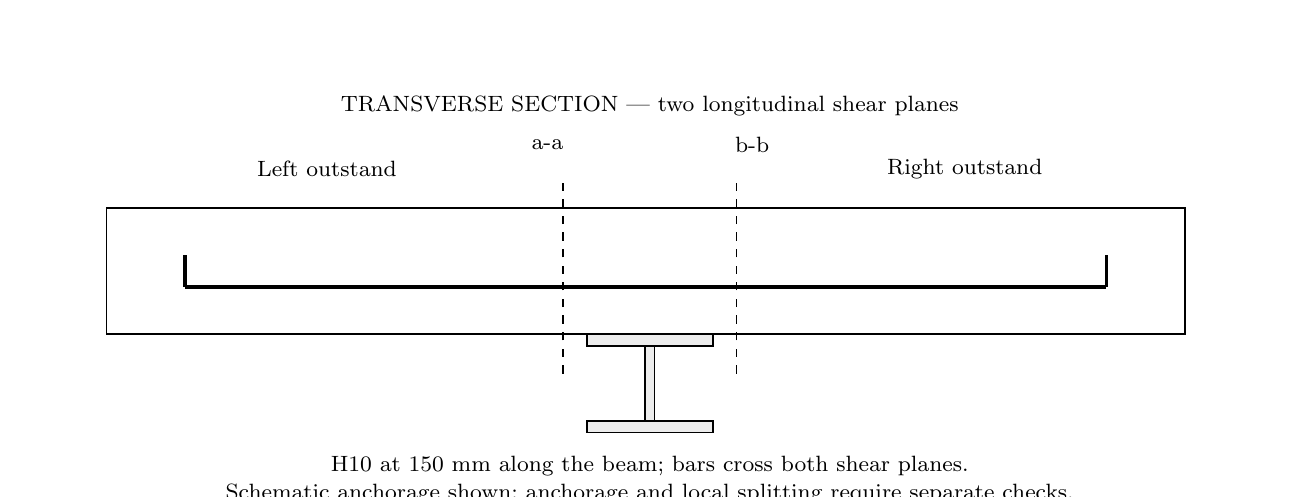
\begin{tikzpicture}[x=1cm,y=1cm,line width=.6pt,>=stealth,font=\fontsize{8.5}{10}\selectfont]\path[use as bounding box] (0,0) rectangle (15.8,5.6);\node at (7.9,5.1){TRANSVERSE SECTION — two longitudinal shear planes};\draw (1,2.2) rectangle (14.7,3.8);\draw[fill=gray!15] (7.1,2.05) rectangle (8.7,2.2);\draw[fill=gray!15] (7.84,1.1) rectangle (7.96,2.05);\draw[fill=gray!15] (7.1,.95) rectangle (8.7,1.1);\foreach \x in {6.8,9}{\draw[dashed] (\x,1.7)--(\x,4.2);}\draw[line width=1.2pt] (2,2.8)--(13.7,2.8);\draw[line width=1.2pt] (2,2.8)--(2,3.2);\draw[line width=1.2pt] (13.7,2.8)--(13.7,3.2);\node at (3.8,4.3){Left outstand};\node at (11.9,4.3){Right outstand};\node at (6.6,4.6){a-a};\node at (9.2,4.6){b-b};\node[align=center] at (7.9,.35){H10 at 150 mm along the beam; bars cross both shear planes.\\Schematic anchorage shown; anchorage and local splitting require separate checks.};\end{tikzpicture}\end{minipage}\par\vspace{5pt}

\sect{12. SERVICEABILITY — STAGED LOADS}
{\small\color{muted}EC4 §5.4.2.2: nL = n0 (1 + psiL phi); psiL = 1.1 permanent, 0.55 shrinkage.}\par
{\small\color{muted}Steel carries wet slab and self weight before curing. Formwork/construction loads are removed.}\par
{\small\color{muted}NCCI PN002a §3: unpropped slip correction 0.3(1-eta)(delta\_s-delta\_c), guidance for review.}\par
\Needspace{24mm}\begin{minipage}{\linewidth}{\small\bfseries\color{muted}Modular ratio}\par\vspace{3pt}{\small\eq{n_0\coloneq  \frac{E_a}{E_{cm}}}\par\vspace{2pt}\eq{=\frac{210000\,\mathrm{MPa}}{33000\,\mathrm{MPa}}}\par\vspace{2pt}\eq{\color{navy}=6.364}}\par\vspace{7pt}\end{minipage}\par
\Needspace{24mm}\begin{minipage}{\linewidth}{\small\bfseries\color{muted}Slab transformed area}\par\vspace{3pt}{\small\eq{A_{c.0}\coloneq  \frac{b_{eff}h_c}{n_0}}\par\vspace{2pt}\eq{=\frac{(2\,\mathrm{m})\cdot (0.15\,\mathrm{m})}{6.364}}\par\vspace{2pt}\eq{\color{navy}=47142.857\,\mathrm{mm}^{2}}}\par\vspace{7pt}\end{minipage}\par
\Needspace{24mm}\begin{minipage}{\linewidth}{\small\bfseries\color{muted}Elastic NA depth below slab top}\par\vspace{3pt}{\small\eq{y_0\coloneq  \frac{A_a(h_c+h_a/2)+A_{c.0}h_c/2}{A_a+A_{c.0}}}\par\vspace{2pt}\eq{=\frac{(7650\,\mathrm{mm}^{2})\cdot (0.15\,\mathrm{m}+0.4064\,\mathrm{m}/2)+(0.04714\,\mathrm{m}^{2})\cdot (0.15\,\mathrm{m})/2}{7650\,\mathrm{mm}^{2}+0.04714\,\mathrm{m}^{2}}}\par\vspace{2pt}\eq{\color{navy}=113.841\,\mathrm{mm}}}\par\vspace{7pt}\end{minipage}\par
\Needspace{24mm}\begin{minipage}{\linewidth}{\small\bfseries\color{muted}Transformed second moment}\par\vspace{3pt}{\small\eq{I_0\coloneq  I_a+A_a(h_c+\frac{h_a}{2}-y_0)^2+\frac{b_{eff}h_c^3}{12n_0}+A_{c.0}(y_0-\frac{h_c}{2})^2}\par\vspace{2pt}\eq{=2.16\times10^{8}\,\mathrm{mm}^{4}+(7650\,\mathrm{mm}^{2})\cdot (0.15\,\mathrm{m}+\frac{0.4064\,\mathrm{m}}{2}-0.1138\,\mathrm{m})^{2}+\frac{(2\,\mathrm{m})\cdot (0.15\,\mathrm{m})^{3}}{12\cdot 6.364}+(0.04714\,\mathrm{m}^{2})\cdot (0.1138\,\mathrm{m}-\frac{0.15\,\mathrm{m}}{2})^{2}}\par\vspace{2pt}\eq{\color{navy}=8.138\times10^{8}\,\mathrm{mm}^{4}}}\par\vspace{7pt}\end{minipage}\par
\Needspace{24mm}\begin{minipage}{\linewidth}{\small\bfseries\color{muted}Modular ratio}\par\vspace{3pt}{\small\eq{n_L\coloneq  n_0(1+1.1\varphi)}\par\vspace{2pt}\eq{=6.364(1+1.1\cdot 2)}\par\vspace{2pt}\eq{\color{navy}=20.364}}\par\vspace{7pt}\end{minipage}\par
\Needspace{24mm}\begin{minipage}{\linewidth}{\small\bfseries\color{muted}Slab transformed area}\par\vspace{3pt}{\small\eq{A_{c.L}\coloneq  \frac{b_{eff}h_c}{n_L}}\par\vspace{2pt}\eq{=\frac{(2\,\mathrm{m})\cdot (0.15\,\mathrm{m})}{20.364}}\par\vspace{2pt}\eq{\color{navy}=14732.143\,\mathrm{mm}^{2}}}\par\vspace{7pt}\end{minipage}\par
\Needspace{24mm}\begin{minipage}{\linewidth}{\small\bfseries\color{muted}Elastic NA depth below slab top}\par\vspace{3pt}{\small\eq{y_L\coloneq  \frac{A_a(h_c+h_a/2)+A_{c.L}h_c/2}{A_a+A_{c.L}}}\par\vspace{2pt}\eq{=\frac{(7650\,\mathrm{mm}^{2})\cdot (0.15\,\mathrm{m}+0.4064\,\mathrm{m}/2)+(0.01473\,\mathrm{m}^{2})\cdot (0.15\,\mathrm{m})/2}{7650\,\mathrm{mm}^{2}+0.01473\,\mathrm{m}^{2}}}\par\vspace{2pt}\eq{\color{navy}=170.086\,\mathrm{mm}}}\par\vspace{7pt}\end{minipage}\par
\Needspace{24mm}\begin{minipage}{\linewidth}{\small\bfseries\color{muted}Transformed second moment}\par\vspace{3pt}{\small\eq{I_L\coloneq  I_a+A_a(h_c+\frac{h_a}{2}-y_L)^2+\frac{b_{eff}h_c^3}{12n_L}+A_{c.L}(y_L-\frac{h_c}{2})^2}\par\vspace{2pt}\eq{=2.16\times10^{8}\,\mathrm{mm}^{4}+(7650\,\mathrm{mm}^{2})\cdot (0.15\,\mathrm{m}+\frac{0.4064\,\mathrm{m}}{2}-0.1701\,\mathrm{m})^{2}+\frac{(2\,\mathrm{m})\cdot (0.15\,\mathrm{m})^{3}}{12\cdot 20.364}+(0.01473\,\mathrm{m}^{2})\cdot (0.1701\,\mathrm{m}-\frac{0.15\,\mathrm{m}}{2})^{2}}\par\vspace{2pt}\eq{\color{navy}=6.333\times10^{8}\,\mathrm{mm}^{4}}}\par\vspace{7pt}\end{minipage}\par
\Needspace{24mm}\begin{minipage}{\linewidth}{\small\bfseries\color{muted}Modular ratio}\par\vspace{3pt}{\small\eq{n_s\coloneq  n_0(1+0.55\varphi)}\par\vspace{2pt}\eq{=6.364(1+0.55\cdot 2)}\par\vspace{2pt}\eq{\color{navy}=13.364}}\par\vspace{7pt}\end{minipage}\par
\Needspace{24mm}\begin{minipage}{\linewidth}{\small\bfseries\color{muted}Slab transformed area}\par\vspace{3pt}{\small\eq{A_{c.s}\coloneq  \frac{b_{eff}h_c}{n_s}}\par\vspace{2pt}\eq{=\frac{(2\,\mathrm{m})\cdot (0.15\,\mathrm{m})}{13.364}}\par\vspace{2pt}\eq{\color{navy}=22448.98\,\mathrm{mm}^{2}}}\par\vspace{7pt}\end{minipage}\par
\Needspace{24mm}\begin{minipage}{\linewidth}{\small\bfseries\color{muted}Elastic NA depth below slab top}\par\vspace{3pt}{\small\eq{y_s\coloneq  \frac{A_a(h_c+h_a/2)+A_{c.s}h_c/2}{A_a+A_{c.s}}}\par\vspace{2pt}\eq{=\frac{(7650\,\mathrm{mm}^{2})\cdot (0.15\,\mathrm{m}+0.4064\,\mathrm{m}/2)+(0.02245\,\mathrm{m}^{2})\cdot (0.15\,\mathrm{m})/2}{7650\,\mathrm{mm}^{2}+0.02245\,\mathrm{m}^{2}}}\par\vspace{2pt}\eq{\color{navy}=145.708\,\mathrm{mm}}}\par\vspace{7pt}\end{minipage}\par
\Needspace{24mm}\begin{minipage}{\linewidth}{\small\bfseries\color{muted}Transformed second moment}\par\vspace{3pt}{\small\eq{I_s\coloneq  I_a+A_a(h_c+\frac{h_a}{2}-y_s)^2+\frac{b_{eff}h_c^3}{12n_s}+A_{c.s}(y_s-\frac{h_c}{2})^2}\par\vspace{2pt}\eq{=2.16\times10^{8}\,\mathrm{mm}^{4}+(7650\,\mathrm{mm}^{2})\cdot (0.15\,\mathrm{m}+\frac{0.4064\,\mathrm{m}}{2}-0.1457\,\mathrm{m})^{2}+\frac{(2\,\mathrm{m})\cdot (0.15\,\mathrm{m})^{3}}{12\cdot 13.364}+(0.02245\,\mathrm{m}^{2})\cdot (0.1457\,\mathrm{m}-\frac{0.15\,\mathrm{m}}{2})^{2}}\par\vspace{2pt}\eq{\color{navy}=6.997\times10^{8}\,\mathrm{mm}^{4}}}\par\vspace{7pt}\end{minipage}\par
\Needspace{24mm}\begin{minipage}{\linewidth}{\small\bfseries\color{muted}Permanent locked-in deflection before curing}\par\vspace{3pt}{\small\eq{\delta_g\coloneq  \frac{5(g_a+g_c)L^4}{384E_a I_a}}\par\vspace{2pt}\eq{=\frac{5(0.5896\,\mathrm{kN}/\mathrm{m}+11.25\,\mathrm{kN}/\mathrm{m})(8\,\mathrm{m})^{4}}{384\cdot (210000\,\mathrm{MPa})\cdot (2.16\times10^{8}\,\mathrm{mm}^{4})}}\par\vspace{2pt}\eq{\color{navy}=13.921\,\mathrm{mm}}}\par\vspace{7pt}\end{minipage}\par
\Needspace{24mm}\begin{minipage}{\linewidth}{\small\bfseries\color{muted}Instantaneous post-curing finishes and imposed load}\par\vspace{3pt}{\small\eq{\delta_{post}\coloneq  \frac{5(g_{SDL}+q_k)s_b L^4}{384E_a I_0}}\par\vspace{2pt}\eq{=\frac{5(1.5\,\mathrm{kPa}+3\,\mathrm{kPa})\cdot (3\,\mathrm{m})(8\,\mathrm{m})^{4}}{384\cdot (210000\,\mathrm{MPa})\cdot (8.138\times10^{8}\,\mathrm{mm}^{4})}}\par\vspace{2pt}\eq{\color{navy}=4.213\,\mathrm{mm}}}\par\vspace{7pt}\end{minipage}\par
\Needspace{24mm}\begin{minipage}{\linewidth}{\small\bfseries\color{muted}Long-term post-curing sustained load}\par\vspace{3pt}{\small\eq{\delta_{LT}\coloneq  \frac{5(g_{SDL}+\psi_2 q_k)s_b L^4}{384E_a I_L}}\par\vspace{2pt}\eq{=\frac{5(1.5\,\mathrm{kPa}+0.3\cdot (3\,\mathrm{kPa}))\cdot (3\,\mathrm{m})(8\,\mathrm{m})^{4}}{384\cdot (210000\,\mathrm{MPa})\cdot (6.333\times10^{8}\,\mathrm{mm}^{4})}}\par\vspace{2pt}\eq{\color{navy}=2.887\,\mathrm{mm}}}\par\vspace{7pt}\end{minipage}\par
\Needspace{24mm}\begin{minipage}{\linewidth}{\small\bfseries\color{muted}Transient part of imposed load}\par\vspace{3pt}{\small\eq{\delta_{tr}\coloneq  \frac{5(1-\psi_2)q_k s_b L^4}{384E_a I_0}}\par\vspace{2pt}\eq{=\frac{5(1-0.3)\cdot (3\,\mathrm{kPa})\cdot (3\,\mathrm{m})(8\,\mathrm{m})^{4}}{384\cdot (210000\,\mathrm{MPa})\cdot (8.138\times10^{8}\,\mathrm{mm}^{4})}}\par\vspace{2pt}\eq{\color{navy}=1.966\,\mathrm{mm}}}\par\vspace{7pt}\end{minipage}\par
\Needspace{24mm}\begin{minipage}{\linewidth}{\small\bfseries\color{muted}Free-shrinkage equivalent concrete force}\par\vspace{3pt}{\small\eq{N_{sh}\coloneq  \frac{E_a}{n_s}b_{eff}h_c\varepsilon_{cs}}\par\vspace{2pt}\eq{=\frac{210000\,\mathrm{MPa}}{13.364}\cdot (2\,\mathrm{m})\cdot (0.15\,\mathrm{m})\cdot 0.0003}\par\vspace{2pt}\eq{\color{navy}=1414.286\,\mathrm{kN}}}\par\vspace{7pt}\end{minipage}\par
\Needspace{24mm}\begin{minipage}{\linewidth}{\small\bfseries\color{muted}Shrinkage curvature magnitude, elastic eigenstrain equilibrium}\par\vspace{3pt}{\small\eq{\kappa_{sh}\coloneq  \frac{N_{sh}(y_s-h_c/2)}{E_a I_s}}\par\vspace{2pt}\eq{=\frac{(1414.286\,\mathrm{kN})\cdot (0.1457\,\mathrm{m}-0.15\,\mathrm{m}/2)}{(210000\,\mathrm{MPa})\cdot (6.997\times10^{8}\,\mathrm{mm}^{4})}}\par\vspace{2pt}\eq{\color{navy}=0.0006806\,\mathrm{m}^{-1}}}\par\vspace{7pt}\end{minipage}\par
\Needspace{24mm}\begin{minipage}{\linewidth}{\small\bfseries\color{muted}Uniform shrinkage curvature deflection}\par\vspace{3pt}{\small\eq{\delta_{sh}\coloneq  \frac{\kappa_{sh}L^2}{8}}\par\vspace{2pt}\eq{=\frac{(0.0006806\,\mathrm{m}^{-1})\cdot (8\,\mathrm{m})^{2}}{8}}\par\vspace{2pt}\eq{\color{navy}=5.445\,\mathrm{mm}}}\par\vspace{7pt}\end{minipage}\par
\Needspace{24mm}\begin{minipage}{\linewidth}{\small\bfseries\color{muted}Post-curing steel-only deflection for the same sustained / transient loads}\par\vspace{3pt}{\small\eq{\delta_{a.post}\coloneq  \frac{5(g_{SDL}+q_k)s_b L^4}{384E_a I_a}}\par\vspace{2pt}\eq{=\frac{5(1.5\,\mathrm{kPa}+3\,\mathrm{kPa})\cdot (3\,\mathrm{m})(8\,\mathrm{m})^{4}}{384\cdot (210000\,\mathrm{MPa})\cdot (2.16\times10^{8}\,\mathrm{mm}^{4})}}\par\vspace{2pt}\eq{\color{navy}=15.873\,\mathrm{mm}}}\par\vspace{7pt}\end{minipage}\par
\Needspace{24mm}\begin{minipage}{\linewidth}{\small\bfseries\color{muted}Unpropped slip allowance, NCCI guidance, not an SS EN NA rule}\par\vspace{3pt}{\small\eq{\delta_{slip}\coloneq  0.3(1-\eta)(\delta_{a.post}-\delta_{LT}-\delta_{tr})}\par\vspace{2pt}\eq{=0.3(1-0.7216)(0.01587\,\mathrm{m}-0.002887\,\mathrm{m}-0.001966\,\mathrm{m})}\par\vspace{2pt}\eq{\color{navy}=0.9203\,\mathrm{mm}}}\par\vspace{7pt}\end{minipage}\par
\Needspace{24mm}\begin{minipage}{\linewidth}{\small\bfseries\color{muted}Long-term total plus full live load, no camber}\par\vspace{3pt}{\small\eq{\delta_{tot}\coloneq  \delta_g+\delta_{LT}+\delta_{tr}+\delta_{slip}+\delta_{sh}}\par\vspace{2pt}\eq{=0.01392\,\mathrm{m}+0.002887\,\mathrm{m}+0.001966\,\mathrm{m}+0.0009203\,\mathrm{m}+0.005445\,\mathrm{m}}\par\vspace{2pt}\eq{\color{navy}=25.139\,\mathrm{mm}}}\par\vspace{7pt}\end{minipage}\par
\Needspace{24mm}\begin{minipage}{\linewidth}{\small\bfseries\color{muted}Total deflection with NCCI slip allowance}\par\vspace{3pt}{\small\eq{\mathrm{UR}_{d.2}\coloneq  \frac{\delta_{tot}}{\delta_{lim}}}\par\vspace{2pt}\eq{=\frac{0.02514\,\mathrm{m}}{0.032\,\mathrm{m}}}\par\vspace{2pt}\eq{\color{navy}=0.7856}}\par\vspace{7pt}\end{minipage}\par
\Needspace{25mm}\begin{longtable}{@{}p{0.53\linewidth}p{0.43\linewidth}@{}}\rowcolor{light}{\small Acceptance} & {\small $\mathrm{UR}_{\mathrm{d.2}}=0.7856\;\le\;1\quad\text{\color{pass}PASS}$}\\[5pt]\end{longtable}\Needspace{24mm}\begin{minipage}{\linewidth}{\small\bfseries\color{muted}Long-term slab bottom stress from sustained post-curing load}\par\vspace{3pt}{\small\eq{\sigma_{c.bot}\coloneq  \frac{(g_{SDL}+\psi_2 q_k)s_b L^2(y_L-h_c)}{8n_L I_L}}\par\vspace{2pt}\eq{=\frac{(1.5\,\mathrm{kPa}+0.3\cdot (3\,\mathrm{kPa}))\cdot (3\,\mathrm{m})(8\,\mathrm{m})^{2}(0.1701\,\mathrm{m}-0.15\,\mathrm{m})}{8\cdot 20.364\cdot (6.333\times10^{8}\,\mathrm{mm}^{4})}}\par\vspace{2pt}\eq{\color{navy}=0.08971\,\mathrm{MPa}}}\par\vspace{7pt}\end{minipage}\par

{\small\color{muted}Positive stress above denotes compression. Tension requires cracked-section / crack-width review.}\par
{\small\color{muted}Shrinkage input needs RH, notional size, curing and ages from EC2 §3.1.4 / Annex B.}\par
{\small\color{muted}Final SLS approval requires adopted slip guidance, shrinkage history and stress/cracking review.}\par
\Needspace{65mm}\begin{minipage}{\linewidth}\vspace{4pt}{\bfseries\color{navy}D11 — Stage-dependent deflections; construction set remains after curing}\par

\centering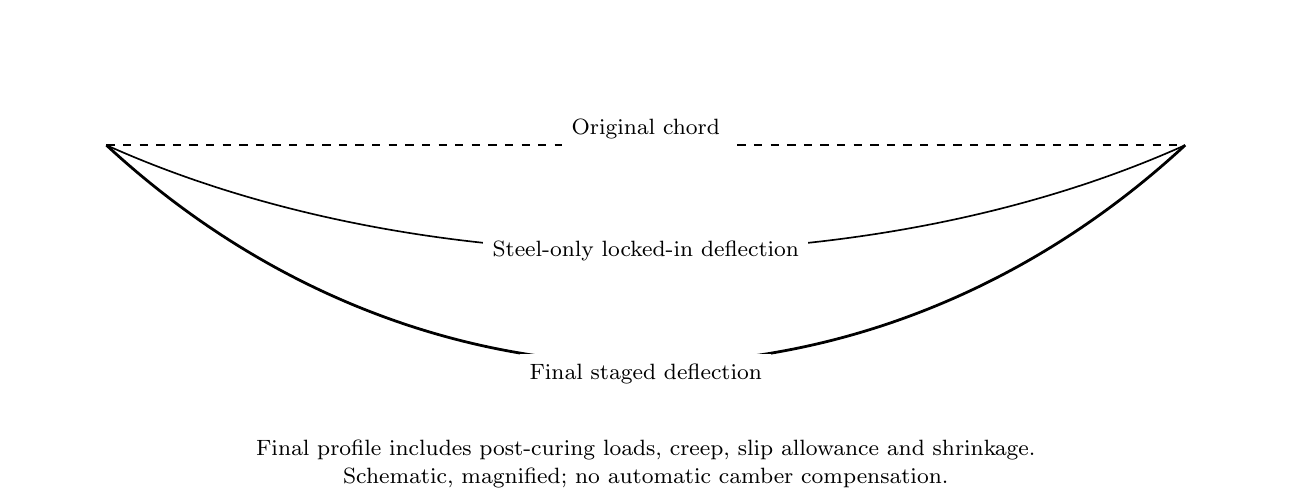
\begin{tikzpicture}[x=1cm,y=1cm,line width=.6pt,>=stealth,font=\fontsize{8.5}{10}\selectfont]\path[use as bounding box] (0,0) rectangle (15.8,5.6);\draw[dashed] (1,4.6)--(14.7,4.6);\draw (1,4.6) .. controls (5,2.8) and (10.7,2.8) .. (14.7,4.6);\draw[line width=1pt] (1,4.6) .. controls (5,.9) and (10.7,.9) .. (14.7,4.6);\node[fill=white] at (7.85,4.8){Original chord};\node[fill=white] at (7.85,3.25){Steel-only locked-in deflection};\node[fill=white] at (7.85,1.7){Final staged deflection};\node[align=center] at (7.85,.55){Final profile includes post-curing loads, creep, slip allowance and shrinkage.\\Schematic, magnified; no automatic camber compensation.};\end{tikzpicture}\end{minipage}\par\vspace{5pt}

\sect{13. DESIGN SUMMARY AND REVIEW GATES}
\Needspace{25mm}\begin{longtable}{@{}p{0.53\linewidth}p{0.43\linewidth}@{}}\rowcolor{light}\textbf{Parameter / reference} & \textbf{Definition / value}\\\midrule
{\small Construction bending} & {\small $\mathrm{UR}_{M.1}=0.4016$}\\[5pt]
{\small Construction vertical shear} & {\small $\mathrm{UR}_{V.1}=0.1207$}\\[5pt]
{\small Construction lateral-torsional buckling} & {\small $\mathrm{UR}_{LT}=1.874$}\\[5pt]
{\small Construction deflection} & {\small $\mathrm{UR}_{d.1}=0.5728$}\\[5pt]
{\small Composite bending} & {\small $\mathrm{UR}_{M.2}=0.3883$}\\[5pt]
{\small Composite vertical shear} & {\small $\mathrm{UR}_{V.2}=0.2007$}\\[5pt]
{\small Transverse reinforcement} & {\small $\mathrm{UR}_{sf}=1.076$}\\[5pt]
{\small Concrete longitudinal shear} & {\small $\mathrm{UR}_{L}=0.7733$}\\[5pt]
{\small Final staged deflection} & {\small $\mathrm{UR}_{d.2}=0.7856$}\\[5pt]\bottomrule\end{longtable}
{\small\color{muted}STATUS: REVIEW DRAFT. LTB and transverse reinforcement failures are retained, not waived.}\par
{\small\color{muted}Release gates: Singapore NAs; staged shrinkage/creep; SLS slip; local splitting/anchorage; welds.}\par
{\small\color{muted}The main bending calculation applies to the verified full-connection slab-PNA branch only.}\par
{\small\color{muted}General steel-PNA equations are annex derivations, not an implemented automatic branch solver.}\par
{\small\color{navy}Annex: References and independent verification}\par
\clearpage
\Needspace{22mm}\vspace{8pt}{\Large\bfseries\color{navy}ANNEX}\par
\sect{General plastic equilibrium and admissible PNA branches}
\Needspace{22mm}\vspace{8pt}{\normalsize\bfseries\color{navy}A.1 General force model — y measured down from top of steel}\par
{\small\color{muted}Width w\_a(y) includes root fillets from the chosen section; Aa and Wpl alone do not locate PNA.}\par
\Needspace{25mm}\begin{longtable}{@{}p{0.53\linewidth}p{0.43\linewidth}@{}}\rowcolor{light}\textbf{Parameter / reference} & \textbf{Definition / value}\\\midrule
{\small Compressed steel area above steel PNA} & {\small $A_{ac}(y)=\int_0^y w_a(z)\,\mathrm{d}z$}\\[5pt]
{\small Equilibrium for available concrete force} & {\small $2f_{yd}A_{ac}(y_a)+N_c=A_a f_{yd}$}\\[5pt]
{\small Compressed steel first moment about slab top} & {\small $Q_{ac}(y)=\int_0^y\left(h_c+z\right)w_a(z)\,\mathrm{d}z$}\\[5pt]
{\small Common-axis moment equilibrium; concrete centroid at xc/2} & {\small $M_{Rd}=f_{yd}A_a\left(h_c+\frac{h_a}{2}\right)-2f_{yd}Q_{ac}(y_a)-\frac{N_c x_c}{2}$}\\[5pt]\bottomrule\end{longtable}
{\small\color{muted}This direct stress-block solution is a reference derivation; main design uses linear interaction.}\par
\Needspace{22mm}\vspace{8pt}{\normalsize\bfseries\color{navy}A.2 Admissible steel PNA branches}\par
{\small\color{muted}Top flange: 0 <= Aac <= ba tf; ya = Aac/ba. Root fillet transition follows flange.}\par
{\small\color{muted}Web: after flange and fillet area; solve cumulative actual steel area above ya.}\par
{\small\color{muted}For a sharp-corner I only: ya = tf + (Aac - ba tf)/tw in the web.}\par
{\small\color{muted}Do not combine the sharp-corner formula with rolled section area including fillets.}\par
{\small\color{muted}At Nc >= 0 and zero applied axial force, Aac <= Aa/2: steel PNA cannot pass mid-depth.}\par
{\small\color{muted}Lower flange is inadmissible for this symmetric, sagging, zero-axial-force configuration.}\par
\Needspace{65mm}\begin{minipage}{\linewidth}\vspace{4pt}{\bfseries\color{navy}D06 — Admissible branch: steel PNA in upper flange}\par

\centering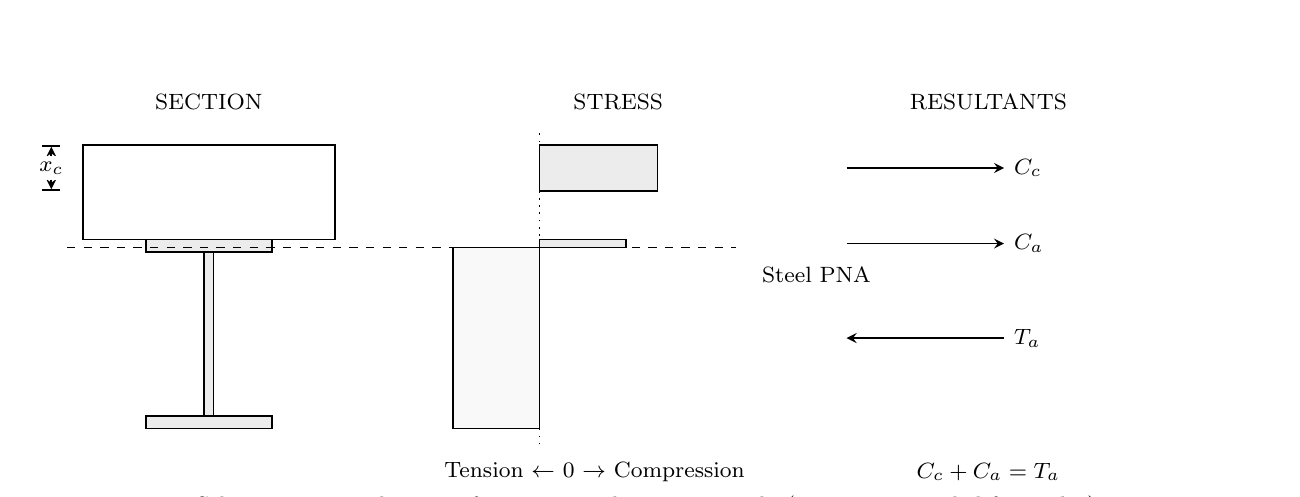
\begin{tikzpicture}[x=1cm,y=1cm,line width=.6pt,>=stealth,font=\fontsize{8.5}{10}\selectfont]\path[use as bounding box] (0,0) rectangle (15.8,5.6);\draw[fill=gray!15] (1.5,1) rectangle ++(1.6,.16);\draw[fill=gray!15] (2.24,1.16) rectangle ++(.12,2.08);\draw[fill=gray!15] (1.5,3.24) rectangle ++(1.6,.16);\draw (0.7,3.4) rectangle (3.9,4.6);\node at (2.3,5.15){SECTION};\node at (7.5,5.15){STRESS};\node at (12.2,5.15){RESULTANTS};\draw[dashed] (.5,3.3)--(9,3.3);\node[anchor=west] at (9.2,2.95){Steel PNA};\draw[dotted] (6.5,.8)--(6.5,4.8);\draw[fill=gray!15] (6.5,4.02) rectangle (8,4.6);\draw[->] (10.4,4.31)--(12.4,4.31) node[right]{$C_c$};\draw[fill=gray!15] (6.5,3.3) rectangle (7.6,3.4);\draw[->] (10.4,3.3499999999999996)--(12.4,3.3499999999999996) node[right]{$C_a$};\draw[fill=gray!5] (5.4,1) rectangle (6.5,3.3);\draw[<-] (10.4,2.15)--(12.4,2.15) node[right]{$T_a$};\node at (7.2,.45){Tension $\leftarrow$ 0 $\rightarrow$ Compression};\node at (12.2,.45){$C_c+C_a=T_a$};\draw[|<->|] (0.3,4.02)--(0.3,4.6) node[midway,fill=white,inner sep=2pt]{$x_c$};\node at (7.9,0){Schematic stress diagram; force arrows shown separately (not an area-scaled force plot).};\end{tikzpicture}\end{minipage}\par\vspace{5pt}

\Needspace{65mm}\begin{minipage}{\linewidth}\vspace{4pt}{\bfseries\color{navy}D07 — Admissible branch: steel PNA in upper web}\par

\centering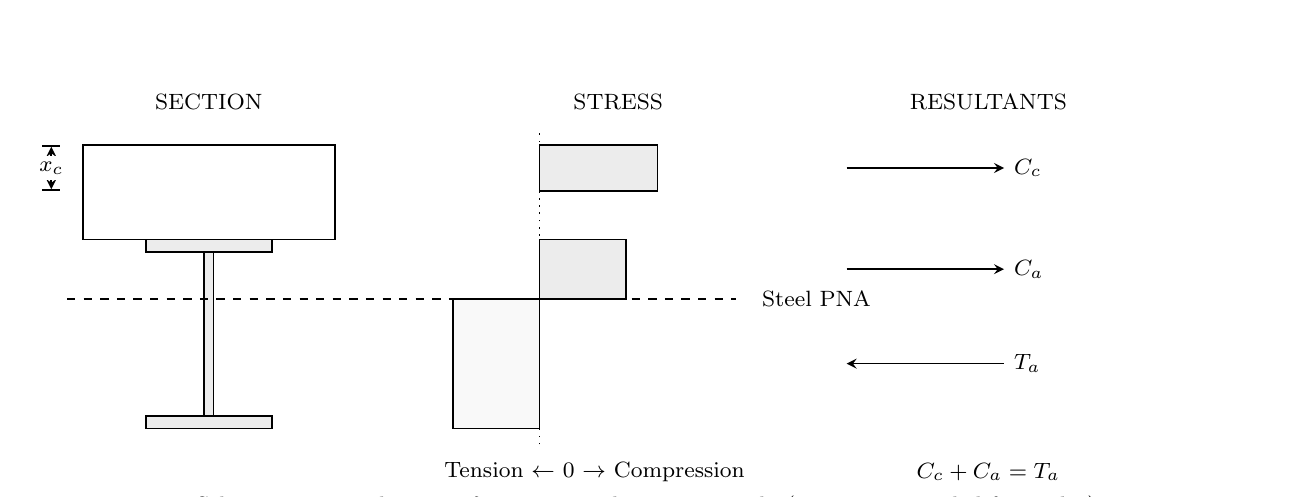
\begin{tikzpicture}[x=1cm,y=1cm,line width=.6pt,>=stealth,font=\fontsize{8.5}{10}\selectfont]\path[use as bounding box] (0,0) rectangle (15.8,5.6);\draw[fill=gray!15] (1.5,1) rectangle ++(1.6,.16);\draw[fill=gray!15] (2.24,1.16) rectangle ++(.12,2.08);\draw[fill=gray!15] (1.5,3.24) rectangle ++(1.6,.16);\draw (0.7,3.4) rectangle (3.9,4.6);\node at (2.3,5.15){SECTION};\node at (7.5,5.15){STRESS};\node at (12.2,5.15){RESULTANTS};\draw[dashed] (.5,2.65)--(9,2.65);\node[anchor=west] at (9.2,2.65){Steel PNA};\draw[dotted] (6.5,.8)--(6.5,4.8);\draw[fill=gray!15] (6.5,4.02) rectangle (8,4.6);\draw[->] (10.4,4.31)--(12.4,4.31) node[right]{$C_c$};\draw[fill=gray!15] (6.5,2.65) rectangle (7.6,3.4);\draw[->] (10.4,3.025)--(12.4,3.025) node[right]{$C_a$};\draw[fill=gray!5] (5.4,1) rectangle (6.5,2.65);\draw[<-] (10.4,1.825)--(12.4,1.825) node[right]{$T_a$};\node at (7.2,.45){Tension $\leftarrow$ 0 $\rightarrow$ Compression};\node at (12.2,.45){$C_c+C_a=T_a$};\draw[|<->|] (0.3,4.02)--(0.3,4.6) node[midway,fill=white,inner sep=2pt]{$x_c$};\node at (7.9,0){Schematic stress diagram; force arrows shown separately (not an area-scaled force plot).};\end{tikzpicture}\end{minipage}\par\vspace{5pt}

\Needspace{65mm}\begin{minipage}{\linewidth}\vspace{4pt}{\bfseries\color{navy}D08 — Lower-flange PNA rejected by force equilibrium}\par

\centering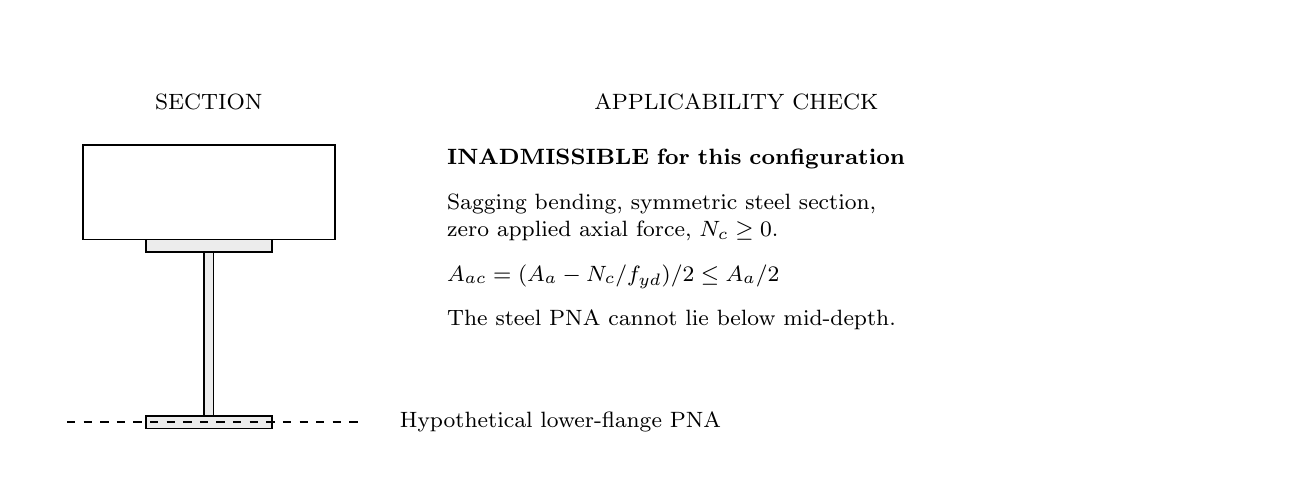
\begin{tikzpicture}[x=1cm,y=1cm,line width=.6pt,>=stealth,font=\fontsize{8.5}{10}\selectfont]\path[use as bounding box] (0,0) rectangle (15.8,5.6);\draw[fill=gray!15] (1.5,1) rectangle ++(1.6,.16);\draw[fill=gray!15] (2.24,1.16) rectangle ++(.12,2.08);\draw[fill=gray!15] (1.5,3.24) rectangle ++(1.6,.16);\draw (0.7,3.4) rectangle (3.9,4.6);\node at (2.3,5.15){SECTION};\node at (9,5.15){APPLICABILITY CHECK};\draw[dashed] (.5,1.08)--(4.2,1.08);\node[anchor=west] at (4.6,1.08){Hypothetical lower-flange PNA};\node[align=left,text width=8cm,anchor=west] at (5.2,3.4){\textbf{INADMISSIBLE for this configuration}\\[6pt]Sagging bending, symmetric steel section,\\zero applied axial force, $N_c\geq0$.\\[6pt]$A_{ac}=(A_a-N_c/f_{yd})/2\leq A_a/2$\\[6pt]The steel PNA cannot lie below mid-depth.};\end{tikzpicture}\end{minipage}\par\vspace{5pt}

\sect{References and scope of independent verification}
{\small\color{muted}SCI / European steel partners: Steel Buildings in Europe, Part 10, Technical Software Specification.}\par
{\small\color{muted}SCI P364, Steel Building Design: Worked Examples, Example 8 — independent methodology check.}\par
{\small\color{muted}SCI section tables / Steel Designers Manual: UB 406 x 178 x 60; rounded published properties.}\par
{\small\color{muted}SCI NCCI SN003b: Mcr and UDL C1/C2; fork supports and top-flange loading.}\par
{\small\color{muted}EC4 §§5.4.1.2, 5.4.2.2, 6.2.1.2, 6.2.1.3, 6.2.2.4, 6.6, 7.3.1.}\par
{\small\color{muted}EC3 §§5.5, 6.2.5, 6.2.6, 6.2.8, 6.3.2.2; EC2 §§3.1.4, 6.2.4 and anchorage provisions.}\par
{\small\color{muted}BCA Approved Document requires the relevant Singapore National Annexes. Factors remain gated.}\par
{\small\color{muted}This project example is calculated independently; it is not a reproduced published benchmark.}\par
\end{document}